\documentclass[12pt,a4paper]{article}
% Fix for fancyhdr headheight error
\setlength{\headheight}{14.5pt}
% --- PACKAGES ---
% --- ENCODING & FONTS ---
\usepackage[utf8]{inputenc}
\usepackage[T1]{fontenc}
\usepackage{lmodern}          % Modern font (alternative to Times)
% \usepackage{times}          % OPTIONAL: Classic serif font (comment if using lmodern)

\usepackage{pgf-pie}
\usepackage{pgfplots}
\usepackage{subcaption}
\usepackage{xcolor}
\usepackage{colortbl}
\usepackage{multirow}
\usepackage{booktabs}
\usepackage{siunitx}
\usepackage{float}

% --- PAGE LAYOUT ---
\usepackage[a4paper, left=0.75in, right=0.75in, top=1in, bottom=1in]{geometry}
\usepackage{parskip}          % Paragraphs with spacing instead of indentation
\usepackage{setspace}         % For line spacing

% --- MATHEMATICS ---
\usepackage{amsmath, amsfonts, amssymb}

% --- GRAPHICS & FIGURES ---
\usepackage{graphicx}
\usepackage{caption, subcaption}
\usepackage{float}
\usepackage{booktabs}         % Better tables
\usepackage{array, longtable, colortbl}
\usepackage{multirow}         % Multirow cells in tables

% --- COLORS ---
\usepackage[table]{xcolor}
\usepackage{xcolor}           % General color usage

% --- TIKZ & DIAGRAMS ---
\usepackage{tikz}
\usetikzlibrary{
  shapes.geometric,
  arrows.meta,
  positioning,
  fit,
  backgrounds,
  shapes.multipart
}

% --- PLOTS & CHARTS ---
\usepackage{pgf-pie}          % Pie charts
\usepackage{pgfplots}         % Graphs and plots
% Set pgfplots compatibility for modern features
\pgfplotsset{compat=1.18}

% --- DOCUMENT STRUCTURE ---
\usepackage{titlesec}         % Custom section titles
\usepackage{tocloft}          % Table of contents formatting
\usepackage{enumitem}         % Better lists

% --- HEADER, FOOTER & LINKS ---
\usepackage{fancyhdr}         % Custom headers/footers

% --- BIBLIOGRAPHY ---
\usepackage[numbers,sort&compress]{natbib}  % For references with numerical citations
\bibliographystyle{plainnat}  % Compatible style with natbib

% --- Load hyperref last ---
\usepackage{hyperref}         % Clickable links




% --- COLORS ---
\definecolor{RoyalBlue}{RGB}{0, 70, 140}
\definecolor{RUETRed}{RGB}{179, 0, 0}
\definecolor{LightGray}{RGB}{248, 249, 250}
\definecolor{DarkGray}{RGB}{52, 58, 64}
\definecolor{AccentBlue}{RGB}{13, 110, 253}
\definecolor{ModernGray}{RGB}{108, 117, 125}
\definecolor{lightgreen}{RGB}{200, 255, 200}
\definecolor{lightred}{RGB}{255, 200, 200}

% Define modern color palette
\definecolor{primary}{RGB}{41, 128, 185}
\definecolor{secondary}{RGB}{52, 152, 219}
\definecolor{accent}{RGB}{231, 76, 60}
\definecolor{success}{RGB}{46, 204, 113}
\definecolor{warning}{RGB}{241, 196, 15}
\definecolor{darkgray}{RGB}{52, 73, 94}
\definecolor{lightgray}{RGB}{236, 240, 241}
\definecolor{purple}{RGB}{155, 89, 182}
\definecolor{orange}{RGB}{230, 126, 34}
\definecolor{teal}{RGB}{26, 188, 156}


% \definecolor{primary}{RGB}{54, 162, 235}
% \definecolor{accent}{RGB}{255, 99, 132}
% \definecolor{warning}{RGB}{255, 206, 86}
% \definecolor{success}{RGB}{75, 192, 192}
% \definecolor{secondary}{RGB}{153, 102, 255}

% --- FONT & STYLING ---
\renewcommand{\familydefault}{\sfdefault}  % Use sans-serif font
\titleformat{\section}{\fontsize{20}{24}\selectfont\bfseries\color{RoyalBlue}}{\thesection}{1em}{}
\titleformat{\subsection}{\fontsize{16}{20}\selectfont\bfseries\color{RoyalBlue}}{\thesubsection}{1em}{}
\titleformat{\subsubsection}{\fontsize{13}{16}\selectfont\bfseries\color{RoyalBlue}}{\thesubsubsection}{1em}{}

% TOC Styling
\renewcommand{\cfttoctitlefont}{\color{black}\Huge\bfseries}
\renewcommand{\cftsecfont}{\color{RoyalBlue}}
\renewcommand{\cftsecpagefont}{\color{RoyalBlue}}
\renewcommand{\cftsubsecfont}{\color{RoyalBlue}}
\renewcommand{\cftsubsecpagefont}{\color{RoyalBlue}}

% Header and Footer
\pagestyle{fancy}
\fancyhf{}
\fancyhead[C]{\textit{Industrial Attachment: Brainstation 23}}
\fancyfoot[C]{\thepage}
\renewcommand{\headrulewidth}{0.4pt}
\renewcommand{\footrulewidth}{0pt}

% Hyperlink Styling
\hypersetup{
    colorlinks=true,
    linkcolor=RoyalBlue,
    filecolor=magenta,
    urlcolor=cyan,
    pdftitle={Industrial Attachment Report},
    pdfpagemode=FullScreen,
    bookmarks=true,
    bookmarksopen=true,
    pdfborder={0 0 0},
}

% --- Define a global style for all plots for consistency ---
\pgfplotsset{
    every axis/.append style={
        axis x line=bottom,
        axis y line=left,
        label style={font=\bfseries},
        title style={font=\large\bfseries, yshift=1em},
        tick label style={font=\small},
        legend style={font=\small, at={(0.5,-0.2)}, anchor=north, legend columns=-1},
    }
}

% Modern title page with geometric design
\newcommand{\maketitlepage}{
    \begin{titlepage}
        \begin{tikzpicture}[remember picture,overlay]
            \fill[RoyalBlue!10] (current page.north west) rectangle ([yshift=-2.2cm]current page.north east);
            \fill[AccentBlue!5] ([yshift=-14cm]current page.north west) rectangle ([yshift=-16.2cm]current page.north east);
            \fill[RoyalBlue!15] ([xshift=2cm,yshift=-2cm]current page.north west) circle (1.2cm);
            \fill[AccentBlue!15] ([xshift=-2cm,yshift=-15.2cm]current page.north east) circle (0.9cm);
        \end{tikzpicture}

        \centering
        \vspace*{0.6cm}

        % Logo
        \begin{tikzpicture}
            \node[circle, draw=RoyalBlue!30, line width=1.5pt, inner sep=6pt] at (0,0) {
                
\includegraphics[width=2.7cm]{RUET_logo.png}
            };
        \end{tikzpicture}

        \vspace{0.6cm}
        {\fontsize{15.5}{17}\selectfont\bfseries\textcolor{RUETRed}{RAJSHAHI UNIVERSITY OF ENGINEERING \& TECHNOLOGY}\par}
        \vspace{0.2cm}
        {\fontsize{13.5}{16}\selectfont\textcolor{DarkGray}{Department of Computer Science and Engineering}\par}

        \vspace{1.5cm}
        % Title Block
        
\begin{tikzpicture}
            \node[rectangle, fill=RoyalBlue!5, rounded corners=12pt, inner sep=12pt, text width=11.5cm, align=center] at (0,0) {
                {\fontsize{21}{24}\selectfont\bfseries\textcolor{RoyalBlue}{Industrial Attachment Report}\par}
                \vspace{0.15cm}
                {\fontsize{16}{20}\selectfont\bfseries\textcolor{DarkGray}{-}\par}
                \vspace{0.15cm}
                {\fontsize{24}{28}\selectfont\bfseries\textcolor{AccentBlue}{"Brainstation 23"}\par}
            };
        \end{tikzpicture}

        \vspace{1.8cm}
        % Submission info
        \begin{minipage}[t]{0.45\textwidth}
            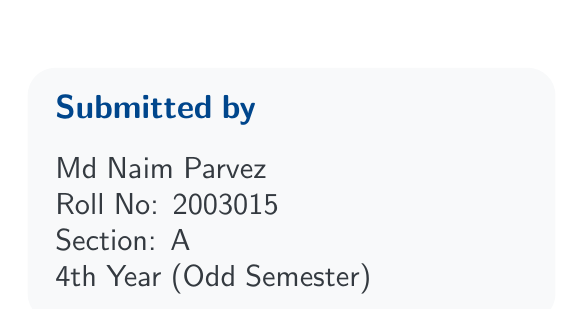
\begin{tikzpicture}
                \node[rectangle, fill=LightGray, rounded corners=10pt, inner sep=10pt, text width=6cm] at (0,0) {
                    {\fontsize{13}{15}\selectfont\bfseries\textcolor{RoyalBlue}{Submitted by}\par}
                    \vspace{0.3cm}
                    {\fontsize{11}{13}\selectfont\textcolor{DarkGray}{
                        Md Naim Parvez\\
                        Roll No: 2003015\\
                        Section: A\\
                        4th Year (Odd Semester)
                    }\par}
                };
            \end{tikzpicture}
        \end{minipage}
        \hfill
        \begin{minipage}[t]{0.50\textwidth}
            
\begin{tikzpicture}
                \node[rectangle, fill=AccentBlue!5, rounded corners=10pt, inner sep=10pt, text width=6cm] at (0,0) {
                    {\fontsize{13}{15}\selectfont\bfseries\textcolor{RoyalBlue}{Submitted to}\par}
                    \vspace{0.3cm}
                    {\fontsize{11}{13}\selectfont\textcolor{DarkGray}{
                        Md. Farhan Shakib\\
                        Lecturer\\
                        Department of CSE\\
                        Rajshahi University of Engineering \& Technology\\
                        \vspace{0.3cm}
                        Signature:\_\_\_\_\_\_\_\_
                    }\par}
                };
            \end{tikzpicture}
        \end{minipage}

        \vspace{1.2cm}
        % Course Info
        
\begin{tikzpicture}
            \node[rectangle, fill=RoyalBlue!10, rounded corners=10pt, inner sep=12pt, align=center, text width=13cm] at (0,0) {
                {\fontsize{13}{16}\selectfont\bfseries\textcolor{RoyalBlue}{Course Code: } \textcolor{DarkGray}{4108}}\\[0.2cm]
                {\fontsize{13}{16}\selectfont\bfseries\textcolor{RoyalBlue}{Course Title: } \textcolor{DarkGray}{Industrial Attachment}}
            };
        \end{tikzpicture}

        \vspace{0.8cm}
    \end{titlepage}
}




\begin{document}

% --- TITLE PAGE ---
\maketitlepage
\thispagestyle{empty} % No header/footer on the title page


\newpage

% --- DECLARATION PAGE ---
\section*{Declaration}
\label{sec:declaration}
\addcontentsline{toc}{section}{Declaration} % Optional: Adds "Declaration" to your Table of Contents
\vspace{3em}
I hereby declare that the work presented in this industrial attachment report, titled \textbf{”Industrial Attachment Experience in Software and AI Development at Brainstation 23”}, is my own original work. It has been completed during my attachment period from [10/03/25] to [25/03/25], 2025.

The information, data, and findings presented in this report are based on my direct experience, observations, and contributions to the projects and activities at Brainstation 23. All sources of information and assistance have been duly acknowledged and referenced.

I confirm that:
\begin{itemize}
    \item This report is the result of my own investigation and effort.
    \item The work has not been previously submitted for any other degree or qualification.
    \item I take full responsibility for the authenticity and accuracy of the content herein.
\end{itemize}

\vspace{5em} % Adds vertical space before the signature lines

\begin{flushleft}
\_\_\_\_\_\_\_\_\_\_\_\_ \\
\textbf{Md. Naim Parvez} \\
Student ID: 2003015 \\
Department of Computer Science and Engineering \\
Rajshahi University of Engineering \& Technology \\
Date: \_\_\_\_\_\_\_\_\_\_

\vspace{3em}

\textbf{Supervisor’s Approval:} \\
\vspace{2em}
\_\_\_\_\_\_\_\_\_\_\_\_ \\
\textbf{Farhan Shakib} \\
Lecturer, Department of CSE \\
Rajshahi University of Engineering \& Technology \\
Date: \_\_\_\_\_\_\_\_\_\_
\end{flushleft}

\newpage

% --- ACKNOWLEDGMENT ---
\section*{Acknowledgment}
\label{sec:acknowledgment}
\addcontentsline{toc}{section}{Acknowledgment} % Add to table of contents
\vspace{3em}
I would like to express my deepest gratitude to my academic supervisor, \textbf{Md. Farhan Shakib}, Lecturer, Department of CSE at Rajshahi University of Engineering \& Technology, for his invaluable guidance and support throughout the course of this industrial attachment.

I am profoundly thankful to \textbf{Brainstation 23} for providing me with the opportunity to undertake my industrial training at their esteemed organization. My sincere appreciation goes to my dedicated corporate supervisors \textbf{Siyam Hossain Ador}, \textbf{Mohaiminul Sohol}, and \textbf{Mehedi Hasan Siddiqee}. Their mentorship, encouragement, and insightful feedback were instrumental in my learning and professional development.

I also wish to extend my special thanks to my team members, \textbf{Sartaj Alam Pritom} and \textbf{Jerin Ramijah Tuli}, for their constant support, collaboration, and for creating a welcoming and conducive work environment. Their cooperation was essential in helping me navigate the challenges and successfully complete my assigned tasks.

Finally, I am grateful to all the staff at Brainstation 23 and the faculty of the CSE department at RUET for their direct and indirect contributions to this enriching experience.

\newpage

\section*{Executive Summary}
\label{sec:executive-summary}
\addcontentsline{toc}{section}{Executive Summary} % Optional: Adds to Table of Contents

This report documents the comprehensive industrial attachment undertaken at \textbf{Brainstation 23}, one of Bangladesh's premier software and technology companies, from [Start Date] to [End Date], 2025. This placement provided an invaluable opportunity to bridge the gap between academic theory and real-world engineering practices, with a deep focus on the rapidly evolving fields of \textbf{Artificial Intelligence, Natural Language Processing, and Full-Stack Web Development}.

Throughout the attachment, I was immersed in a professional, agile environment, contributing to a diverse range of projects that required a blend of specialized AI knowledge and robust software engineering skills. The experience was centered on building end-to-end applications, from conceptual prototypes to fully-featured platforms, providing a holistic view of the modern software development lifecycle.

\paragraph{Key Projects and Achievements} The core of the attachment involved hands-on development of four distinct AI-powered applications. My work began with creating lightweight, API-driven solutions like a \textbf{Conversational AI Chatbot} using OpenRouter and a proof-of-concept \textbf{VisionCare AI Doctor} using Gradio, demonstrating skills in rapid prototyping and third-party API integration.

This foundational work evolved into two more substantial projects. The first, \textbf{SavantSearch}, is a sophisticated semantic search engine that leverages a custom fine-tuned BERT model and a Qdrant vector database to understand natural language queries. The second, and most significant, project was \textbf{AI Doctor Jhatka}, a full-stack medical consultation platform. This system is a major technical achievement, incorporating the LLaVA-7B vision-language model locally via Ollama to ensure data privacy, a secure Flask backend with user authentication, and multimodal interactions (text, voice, and image).

\paragraph{Technical Skills Development} This attachment significantly enhanced my technical skill set. I gained practical experience with a wide array of modern technologies, including:
\begin{itemize}
    \item \textbf{AI and Machine Learning:} Fine-tuning BERT with Triplet Loss, managing vector databases (Qdrant), and deploying local Large Language Models (Llava 7B) with Ollama.
    \item \textbf{Backend Development:} Building scalable web applications using Python, Flask, and the SQLAlchemy ORM for database management.
    \item \textbf{Frontend and UI:} Creating interactive user interfaces with HTML, CSS, JavaScript, and rapid-development frameworks like Streamlit and Gradio.
    \item \textbf{Speech Processing:} Implementing speech-to-text and text-to-speech functionalities using libraries like SpeechRecognition and pyttsx3.
\end{itemize}

\paragraph{Impact and Learning Outcomes} This industrial attachment successfully met its objective of providing deep, practical exposure to professional software engineering. The experience provided profound insights into the complete lifecycle of developing and deploying complex AI applications. Working on a variety of projects sharpened my ability to select the appropriate technology for a given problem, from lean, API-based prototypes to secure, self-hosted platforms. The skills and best practices learned in software architecture, model integration, and project management have built a strong foundation for my future career in the technology industry.

\newpage
% --- TABLE OF CONTENTS ---
\newpage
\pagenumbering{roman} % Roman numerals for ToC, Abstract etc.
\phantomsection % Helps hyperref create proper links
\tableofcontents

% --- LIST OF FIGURES ---
\newpage
\phantomsection % Helps hyperref create proper links
\listoffigures

% % --- LIST OF TABLES ---
% \newpage
% \phantomsection % Helps hyperref create proper links
% \listoftables

% --- LIST OF ABBREVIATIONS ---
\newpage
\phantomsection % Helps hyperref create proper links
\section*{List of Abbreviations}
\label{sec:abbreviations}
\addcontentsline{toc}{section}{List of Abbreviations}

\begin{tabular}{@{}ll@{}}
\toprule
\textbf{Abbreviation} & \textbf{Full Form} \\
\midrule
AI & Artificial Intelligence \\
API & Application Programming Interface \\
CSE & Computer Science and Engineering \\
LLM & Large Language Model \\
RUET & Rajshahi University of Engineering \& Technology \\
ToC & Table of Contents \\
UI & User Interface \\
UX & User Experience \\
SQL & Structured Query Language \\
IDE & Integrated Development Environment \\
IT & Information Technology \\
OS & Operating System \\
HTTP & HyperText Transfer Protocol \\
JSON & JavaScript Object Notation \\
REST & Representational State Transfer \\
CRUD & Create, Read, Update, Delete \\
MVC & Model-View-Controller \\
OOP & Object-Oriented Programming \\
DB & Database \\
DBMS & Database Management System \\
\bottomrule
\end{tabular}

\newpage
\pagenumbering{arabic} % Arabic numerals for main content
\setcounter{page}{1} % Start main content page numbering from 1

% --- MAIN CONTENT ---



% --- CHAPTER 1: INTRODUCTION ---
\section{Introduction}

\subsection{Background of Industrial Attachment}
The industrial attachment is a cornerstone of the undergraduate engineering curriculum, serving as the critical bridge between academic theory and practical, real-world application. This program provides students with an essential transition from a structured academic environment to the dynamic challenges and fast-paced nature of the professional world. With this in mind, I selected Brainstation 23 for my attachment, a decision driven by its prominent status as a top-tier software and technology company in Bangladesh. The company's reputation for technical excellence, innovation, and adherence to industry best practices made it the ideal choice for a comprehensive and impactful learning experience.

A key factor in this decision was Brainstation 23’s diverse and extensive portfolio. Their work spans numerous sectors, including fintech, e-commerce, and healthcare, offering an unparalleled opportunity to observe how fundamental engineering principles are adapted to solve unique, industry-specific problems. This exposure provides a holistic view of the technology landscape and the versatility required of a modern engineer. Furthermore, the company's professional environment is built on a foundation of agile methodologies, close collaboration, and structured mentorship. This culture not only accelerates technical learning but also cultivates critical soft skills such as teamwork, communication, and adaptability, which are vital for a successful career.

The timing of this attachment was also highly relevant, coinciding with a period of significant growth in Bangladesh’s IT sector, which has become a vibrant technological ecosystem. Brainstation 23 stands at the forefront of this wave, actively implementing and innovating with emerging technologies like Artificial Intelligence, Machine Learning, and cloud computing. Being immersed in this forward-thinking environment provided direct exposure to the tools and practices that are shaping the future of the industry. This experience was not just about learning current technologies, but also about understanding the mindset required to continuously adapt and thrive in a field defined by rapid and constant change.

\subsection{Importance in Achieving Engineering Program Outcomes}
This industrial attachment was instrumental in translating academic knowledge into practical engineering competencies. The experience at Brainstation 23 provided a direct line of sight into how a leading technology firm tackles complex problems, thereby solidifying key engineering program outcomes related to problem analysis, solution design, and modern tool usage.

\textbf{From Theory to Production}\\
At Brainstation 23, I moved beyond theoretical exercises to witness the complete lifecycle of production-grade software. I had the unique opportunity to observe the entire process, from initial client requirements gathering to final deployment and ongoing maintenance. Participating in agile ceremonies like daily stand-ups, sprint planning, and code reviews provided a structured, hands-on understanding of how concepts from my software engineering courses are applied in a fast-paced, professional environment. This exposed the true complexity of industry projects, which often involve ambiguous requirements and iterative development—a stark contrast to the well-defined problems in academia.

\textbf{Technical and Collaborative Skills}\\
The experience was deeply collaborative. Working alongside experienced engineers, I learned the importance of effective communication, clear documentation, and version control in achieving project goals. Mentorship from senior developers was invaluable, offering insights into advanced professional practices like writing maintainable code, designing scalable systems, and optimizing for performance. I also gained a practical appreciation for quality assurance, seeing firsthand how automated testing, continuous integration (CI) pipelines, and rigorous peer reviews are essential for delivering robust and reliable software.

\textbf{Integrating Engineering with Business Acumen}\\
Finally, the attachment provided a crucial perspective on the business aspects of technology. I gained an understanding of how engineering solutions must be aligned with client needs and business objectives to be successful. Exposure to processes like project estimation and resource allocation highlighted that technical excellence must be balanced with economic viability. This holistic view, integrating technical skill with business acumen, was one of the most significant learning outcomes of my time at Brainstation 23.

\subsection{Objectives of the Attachment}
The primary objectives for this industrial attachment were carefully formulated to maximize learning outcomes and align with both academic requirements and professional development goals. These objectives were centered on gaining practical skills, professional insight, and a comprehensive understanding of industry practices that would complement and enhance my academic learning.

\textbf{Understanding Project Management Methodologies:} A primary goal was to learn how large-scale technology projects are managed using methodologies like Agile and Scrum. This involved observing the entire project lifecycle, from planning and risk assessment to execution and quality assurance.

\textbf{Collaborative Development Understanding:} I aimed to understand how large teams effectively collaborate on complex projects. This meant gaining practical experience with essential tools and processes like version control (Git), peer code reviews, and team communication protocols.

\textbf{Professional Environment Immersion:} A key objective was to gain firsthand experience in a corporate setting to develop crucial soft skills. This included understanding professional ethics, communication etiquette, and the dynamics of teamwork in a fast-paced environment.

\textbf{Code Quality and Best Practices:} A central technical goal was to learn the principles of writing clean, efficient, and production-grade code. This involved moving beyond academic exercises to focus on code that is maintainable, scalable, and secure.

\textbf{Problem-Solving Skill Development:} I sought to enhance my ability to solve real-world problems. This meant analyzing complex and often ambiguous tasks, researching potential solutions, and implementing effective fixes within large, existing codebases.

\textbf{Technology Integration and Adaptation:} An additional objective emerged during the attachment - learning to integrate and adapt to new technologies quickly. This became particularly relevant as I worked with cutting-edge AI and machine learning technologies, requiring rapid skill acquisition and practical application of emerging tools and frameworks.

\subsection{Scope and Limitations}
The scope of my work during the attachment was primarily focused on the rapidly evolving fields of \textbf{Artificial Intelligence (AI)} and \textbf{Large Language Models (LLM)}, representing some of the most innovative and challenging areas in contemporary software development. This specialization provided deep insights into emerging technologies while also presenting unique learning opportunities and constraints.

\textbf{Technical Scope:} My responsibilities involved developing and integrating AI-powered features into existing applications, requiring a comprehensive understanding of machine learning principles, natural language processing, and AI model deployment strategies. The work encompassed both theoretical understanding and practical implementation of AI solutions, bridging the gap between academic AI concepts and their real-world applications in commercial software products.

Initially, the project work centered on utilizing third-party APIs for model access, which provided valuable experience in API integration, authentication mechanisms, and external service dependency management. This phase involved learning to work with cloud-based AI services, understanding their capabilities and limitations, and developing robust error handling mechanisms for external API interactions. The experience highlighted the importance of designing systems that can gracefully handle external service failures and varying response times.

However, as project requirements evolved, the scope expanded to include implementing local models and integrating them with local databases. This evolution provided deeper technical challenges and more comprehensive learning opportunities, requiring understanding of model optimization, local deployment strategies, and database integration patterns. The transition from cloud-based to local AI implementation offered insights into the trade-offs between computational efficiency, data privacy, and system complexity.

\textbf{Learning Scope:} The scope of learning extended beyond pure technical skills to include understanding the business implications of AI implementations, user experience considerations for AI-powered features, and the ethical considerations surrounding AI deployment in commercial applications. This broader scope provided a holistic view of how technical decisions impact business outcomes and user satisfaction.

\textbf{Limitations:} The primary limitation was the duration of the attachment, which naturally restricted the depth of involvement in long-term project lifecycle phases such as extensive testing, user feedback integration, and post-deployment maintenance. The limited timeframe meant that while I could contribute meaningfully to development phases, the opportunity to observe complete project cycles from conception to long-term maintenance was constrained.

Another significant limitation was the learning curve associated with advanced AI technologies, which required substantial time investment in understanding complex concepts and frameworks. This meant that the initial weeks of the attachment were heavily focused on knowledge acquisition rather than productive contribution, though this investment proved valuable in the latter stages.

The scope was also limited by the specific technologies and frameworks used by the organization, which, while comprehensive, represented only a subset of the available options in the rapidly evolving AI landscape. Additionally, confidentiality requirements restricted the ability to document certain technical implementations and business logic details.

\subsection{Methodology}
The information, experiences, and findings detailed in this report were gathered using a comprehensive, multi-faceted methodology that combined hands-on practical involvement with systematic observation and documentation. This approach was designed to maximize learning outcomes while ensuring accurate and meaningful data collection for analysis and reporting purposes.

\textbf{Direct Project Involvement:} The primary methodological approach involved direct participation in assigned development tasks, allowing for experiential learning through practical application. This hands-on involvement included coding, testing, debugging, and documentation activities that provided firsthand experience with professional software development processes. Each task was approached with careful attention to both the technical implementation and the underlying methodologies and best practices being employed.

\textbf{Systematic Observation:} Daily observation of team workflows, coding practices, and debugging sessions formed a crucial component of the data gathering methodology. This involved maintaining detailed notes on development processes, team interactions, problem-solving approaches, and decision-making patterns observed within the organization. The observational data was systematically categorized to identify patterns, best practices, and areas for improvement.

\textbf{Structured Mentorship Interactions:} Regular meetings with designated supervisors provided opportunities for guided learning and clarification of technical concepts. These sessions were structured to include progress reporting, technical discussions, and strategic planning for upcoming tasks. The mentorship interactions were documented to track learning progression and identify key insights gained through expert guidance.

\textbf{Documentation Review and Analysis:} Comprehensive review of project documentation, including existing codebases, design documents, technical specifications, and architectural guides, provided contextual understanding of project standards and organizational practices. This documentary analysis helped in understanding the historical context of projects and the evolution of technical decisions over time.

\textbf{Collaborative Learning Sessions:} Participation in team meetings, brainstorming sessions, and technical discussions provided insights into collaborative problem-solving methodologies and group decision-making processes. These sessions were particularly valuable for understanding how diverse perspectives contribute to solution development and how consensus is achieved in technical teams.

\textbf{Continuous Reflection and Documentation:} Throughout the attachment period, I maintained a detailed learning journal that captured daily experiences, challenges encountered, solutions developed, and insights gained. This reflective practice ensured that learning was not only experiential but also analytical, promoting deeper understanding of observed phenomena and personal growth patterns.

\subsection{Structure of the Report}
This comprehensive report is systematically organized into ten distinct chapters, each designed to provide detailed insights into different aspects of the industrial attachment experience. The structure follows a logical progression from background information through detailed technical content to conclusions and recommendations.

\textbf{Chapter 1: Introduction} provides a comprehensive foundation for understanding the context, objectives, and methodology of the industrial attachment. This chapter establishes the framework for the entire report and outlines the significance of the experience within the broader context of engineering education.

\textbf{Chapter 2: Organization Overview} presents a detailed examination of Brainstation 23, including its history, organizational structure, business model, technological capabilities, and market position. This chapter provides essential context for understanding the environment in which the attachment took place and the significance of the learning opportunities it provided.

\textbf{Chapter 3: Project Analysis} offers an in-depth exploration of the specific project I was involved in during the attachment. This includes technical specifications, development methodologies, challenges encountered, and solutions implemented. The chapter provides detailed insights into the practical application of engineering principles in a professional setting.

\textbf{Chapter 4: Tools and Technologies} comprehensively covers the software tools, development frameworks, programming languages, and technological platforms utilized during the attachment. This chapter includes analysis of tool selection criteria, implementation strategies, and effectiveness evaluations.

\textbf{Chapters 5 and 6: Societal, Ethical, and Professional Considerations} examine the broader implications of the work undertaken during the attachment, including its impact on society, ethical considerations in AI development, and professional responsibilities in technology implementation. These chapters address the holistic aspects of engineering practice beyond pure technical considerations.

\textbf{Chapter 7: Skills Development and Learning Outcomes} provides a reflective analysis of the competencies gained during the attachment, including both technical skills and professional capabilities. This chapter maps learning outcomes to engineering program objectives and discusses the long-term value of the experience.

\textbf{Chapter 8: Challenges and Solutions} presents a detailed examination of the various obstacles encountered during the attachment and the problem-solving approaches employed to address them. This chapter provides valuable insights into the practical challenges of professional software development and effective solution strategies.

\textbf{Chapter 9: Contributions and Achievements} outlines the specific contributions made to the organization during the attachment period, including technical implementations, process improvements, and knowledge sharing activities. This chapter quantifies the value added through the attachment experience.

\textbf{Chapter 10: Conclusions and Recommendations} synthesizes the key findings from the attachment experience and provides actionable recommendations for future industrial attachments, curriculum improvements, and professional development strategies. This chapter serves as both a summary and a forward-looking analysis of lessons learned.

\newpage
% --- CHAPTER 2: ORGANIZATION OVERVIEW ---
\section{Organization Overview}

\subsection{History and Mission}
Brainstation 23 Limited is a prominent software and technology company based in Dhaka, Bangladesh, founded in 2006 by Raisul Kabir. From its inception, the company has experienced remarkable growth, establishing itself as one of the largest and most reputable software development firms in the country. It has expanded its operations globally, serving clients across various continents, including North America, Europe, and Asia.

The core mission of Brainstation 23 is to provide innovative, high-quality, and cost-effective software solutions to its clients. The company is driven by a passion for technology and a commitment to solving complex business challenges, aiming to be a leading and trusted technology partner for enterprises worldwide.
\begin{figure}[H]
    \centering
    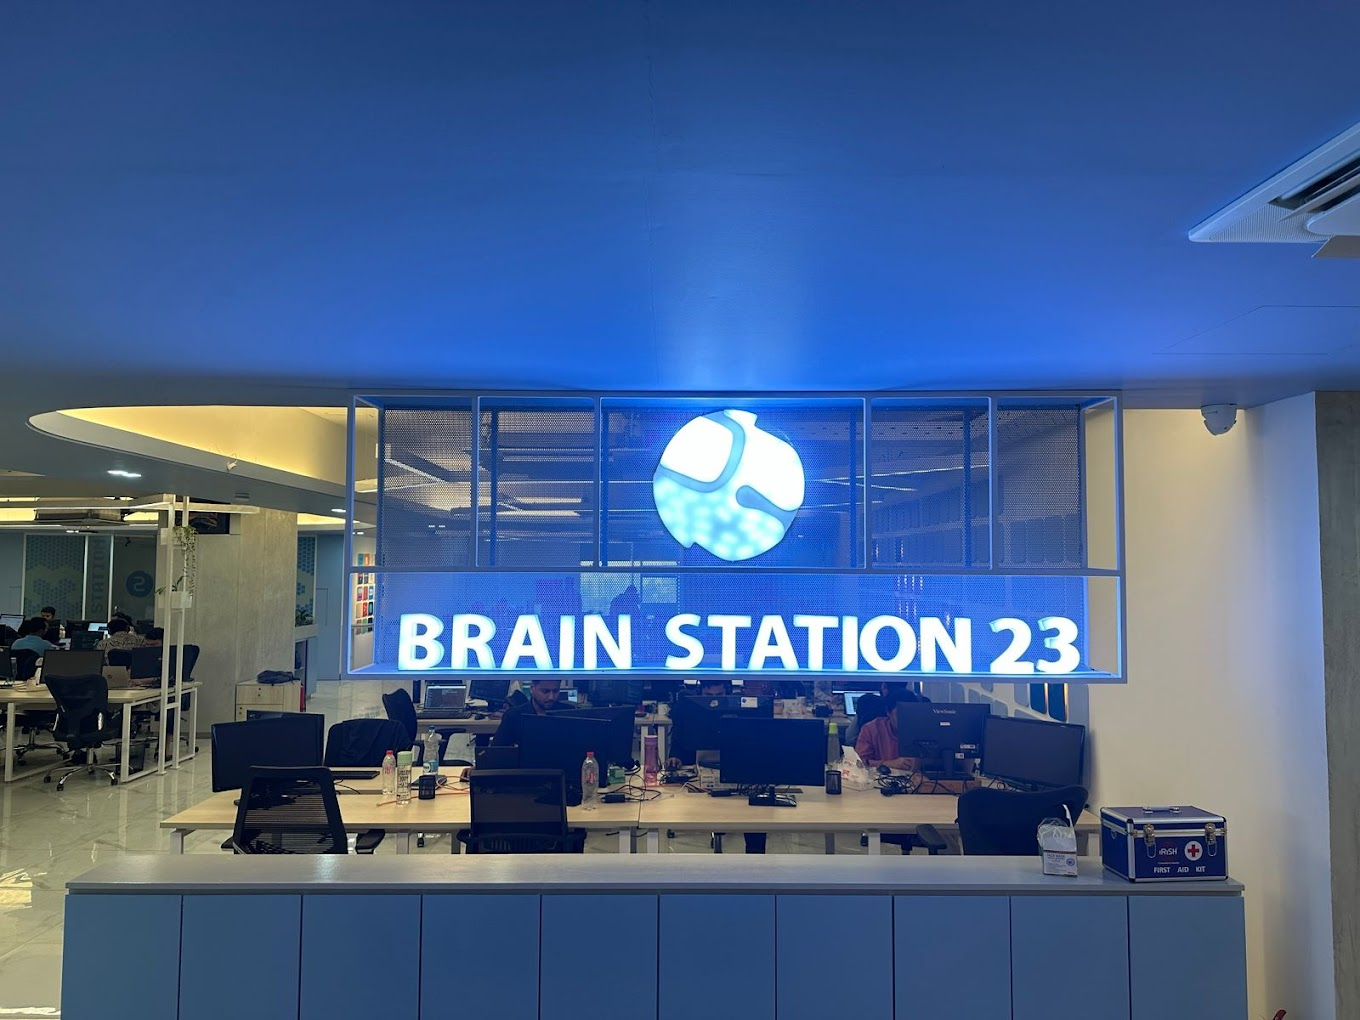
\includegraphics[width=0.5\textwidth]{brain_logo.png}
    \caption{Brainstation 23 Logo}
    \label{fig:brainstation_logo}
\end{figure}

\subsection{Organizational Structure}
The leadership team of Brain Station 23 is composed of its co-founders and senior executives who oversee both the strategic and technical directions of the company. The team includes Raisul Kabir (Chief Executive Officer), who has been guiding the company since its inception in 2006, MJ Ferdous (Chief Operating Officer), who manages day-to-day operations and global market expansion, Mohammad Mizanur Rahman (Chief Technology Officer), responsible for the company’s technology architecture and innovation, Md. Shazedul Hoque (Chief Financial Officer), who oversees financial and administrative functions, and Zubair Ahmed (Chief Sales Officer), leading sales and business development across international markets.

Brain Station 23 maintains a flat and collaborative organizational structure, where ownership and decision-making are distributed among senior leaders and high-performing employees. 

\begin{figure}[H]
    \centering
    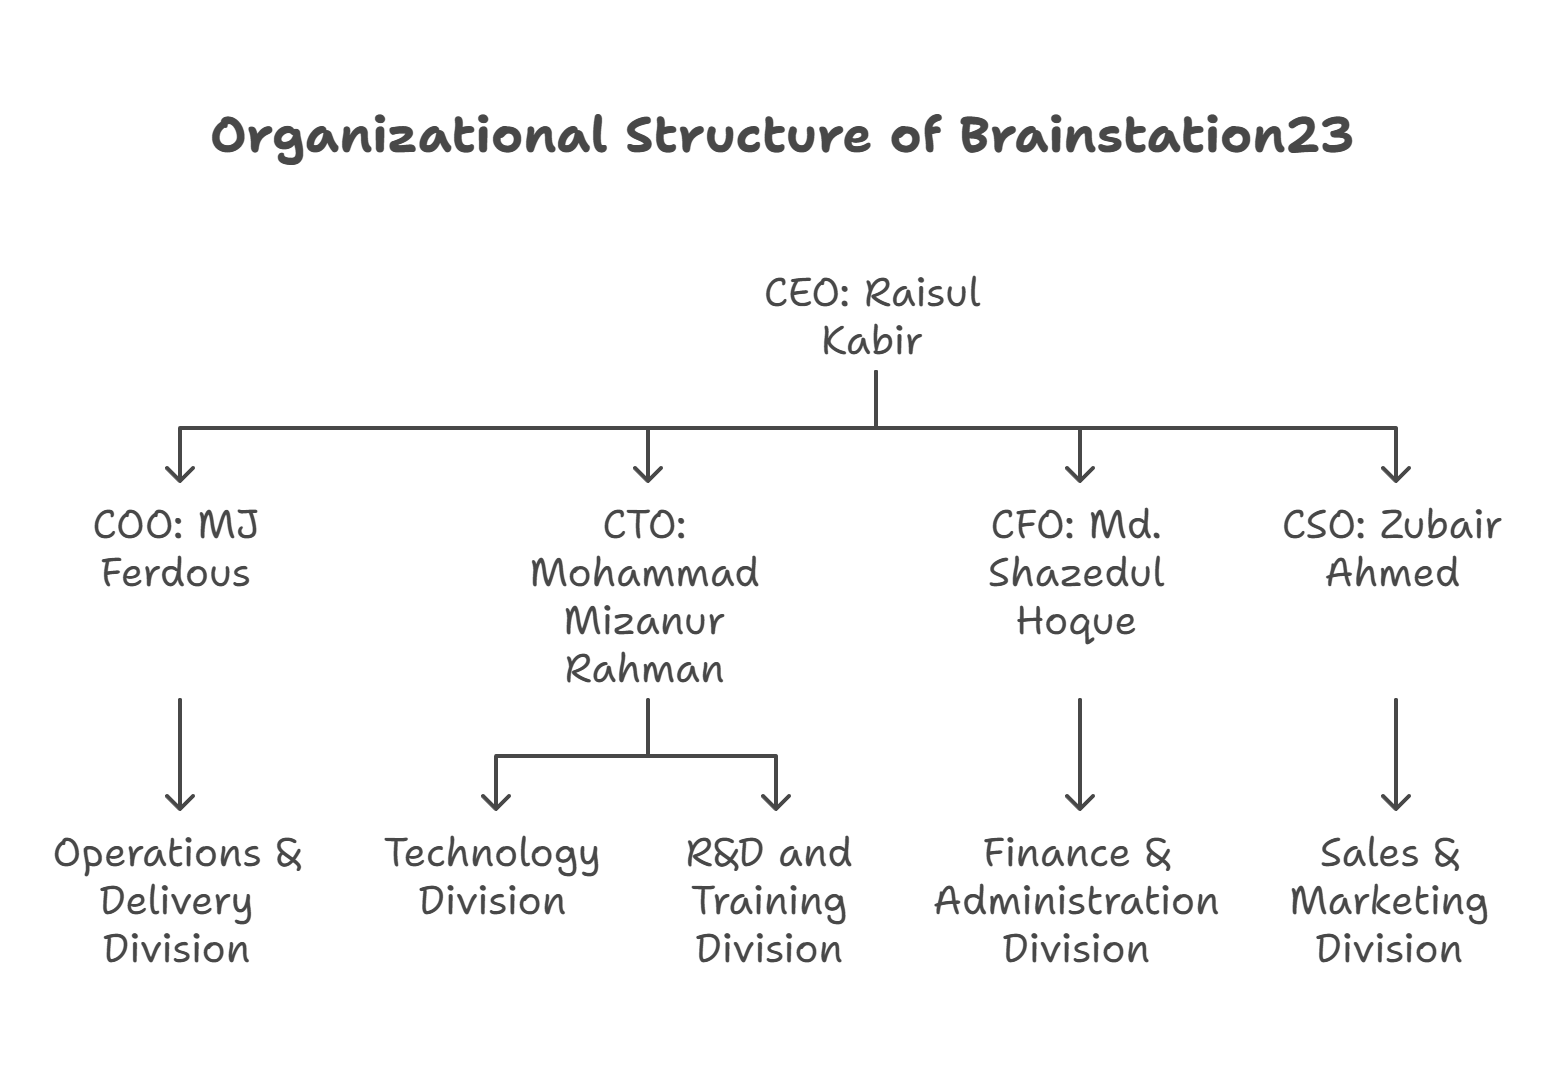
\includegraphics[width=0.8\textwidth]{org_structure.png}
    \caption{Organizational Structure of Brainstation 23}
    \label{fig:org_structure}
\end{figure}

\subsection{Departments and Functions}
Brainstation 23 is composed of several specialized departments, each with distinct functions that contribute to the company's success. The primary departments include:
\begin{itemize}
    \item \textbf{Software Engineering:} The largest department, responsible for the design, development, and maintenance of software, web, and mobile applications. It is further divided into teams based on technology stacks (e.g., .NET, Java, PHP, Python, Mobile).
    
    \item \textbf{Quality Assurance (QA):} Dedicated to ensuring the reliability, performance, and security of products through both manual and automated testing procedures.
    
    \item \textbf{DevOps and Cloud Engineering:} Manages infrastructure automation, CI/CD pipelines, containerization, and cloud deployment (AWS, Azure, GCP) to ensure scalability and efficiency.
    
    \item \textbf{Project Management:} Responsible for planning, monitoring, and delivering projects on time, within budget, and according to client requirements, while coordinating cross-functional teams.
    
    \item \textbf{Business Development \& Sales:} Focuses on acquiring new clients, managing international business partnerships, and driving global expansion across Europe, North America, and the Middle East.
    
    \item \textbf{UI/UX Design:} Ensures that products deliver a user-friendly and visually appealing experience by creating prototypes, wireframes, and user-centered designs.
    
    \item \textbf{Finance and Administration:} Oversees financial planning, budgeting, compliance, and resource management to support overall business operations.
    
    \item \textbf{Human Resources (HR):} Handles recruitment, employee onboarding, training, and continuous professional development programs, while fostering a collaborative workplace culture.
    
    \item \textbf{Artificial Intelligence (AI) \& Machine Learning (ML):} A specialized department focusing on developing solutions in data science, predictive analytics, computer vision, and intelligent automation. This department explores cutting-edge technologies to serve global clients and supports R\&D initiatives.
    
    \item \textbf{Research and Development (R\&D):} Explores emerging technologies such as AR/VR, Blockchain, and Industry 4.0 solutions, ensuring innovation and long-term competitiveness.
    
    \item \textbf{Industry-Specific Divisions:} Dedicated units focusing on Banking and Financial Services, Healthcare, Telecom, E-commerce, and Enterprise Solutions, delivering tailored technical expertise for each domain.
\end{itemize}

\subsection{Products / Services}
Brainstation 23 \citep{brainstation23} offers a comprehensive suite of services and solutions tailored to meet the diverse needs of its clients. Their main service areas include:
\begin{itemize}
    \item Custom Software Development
    \item Web Application Development
    \item Mobile Application Development (iOS, Android, and cross-platform)
    \item Artificial Intelligence \& Machine Learning Solutions
    \item Augmented Reality (AR) \& Virtual Reality (VR)
    \item Blockchain Technology Solutions
    \item Cloud Computing Services (AWS, Azure)
    \item E-commerce and Retail Solutions
    \item Banking and FinTech Solutions
\end{itemize}

\subsection{Quality and Compliance Standards}
Brainstation 23 is committed to maintaining the highest standards of quality in its service delivery. The company employs industry-standard best practices, such as Agile and Scrum methodologies for project management, to ensure iterative development and continuous feedback. They adhere to strict coding standards and conduct regular code reviews to maintain code quality and integrity.

\textbf{Quality Assurance:} The QA department plays a crucial role in the development lifecycle, implementing comprehensive testing strategies that include unit testing, integration testing, system testing, and user acceptance testing (UAT). Automated testing frameworks are also utilized to enhance efficiency and coverage.

Development and maintenance of automated testing suites for web applications, mobile apps, and API services. The department utilizes industry-standard tools such as Selenium, Cypress, and Jest for comprehensive test coverage.

Specialized testing for application performance, scalability, and reliability under various load conditions. This ensures that applications can handle expected user volumes and maintain performance standards.

Regular security assessments, vulnerability scanning, and compliance verification to ensure that applications meet security standards and regulatory requirements.

\textbf{Certifications and Standards:} The company is ISO 9001 certified, demonstrating its commitment to quality management principles. Additionally, Brainstation 23 follows compliance standards relevant to its clients' industries, such as GDPR for data protection and PCI-DSS for payment processing.

\subsection{Project Management and Coordination}
Brainstation 23 employs Agile methodologies, particularly Scrum, to manage its projects. This approach emphasizes iterative development, continuous feedback, and adaptive planning, allowing teams to respond effectively to changing requirements and client needs.

\subsection{Workplace Safety and Environmental Policy}
The company maintains a safe, healthy, and secure work environment for all its employees. This includes ergonomic workstations, a clean office space, and adherence to building safety regulations. The office environment at Brainstation 23 was modern, secure, and well-maintained. Access to the premises was controlled via keycard access, ensuring security for all personnel and assets. The workspace was designed as an open-plan office, fostering collaboration, and was equipped with ergonomic furniture, which reflects the company's commitment to employee well-being and safety.

\begin{figure}[H]
    \centering
    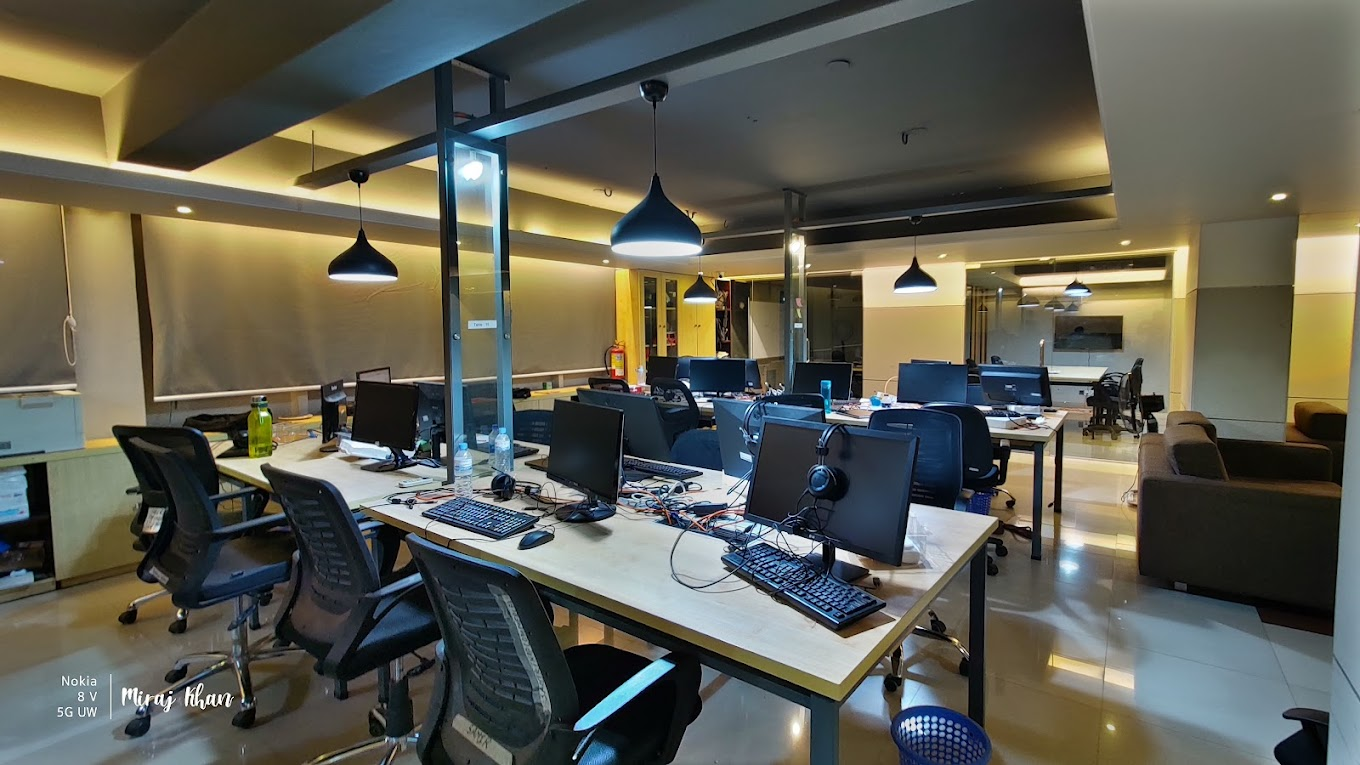
\includegraphics[width=0.85\textwidth]{work_environment.png}
    \caption{Professional Work Environment at Brainstation 23}
    \label{fig:work_environment}
\end{figure}


\newpage
% --- CHAPTER 3: PROJECT OVERVIEW ---
\section{Project Overview}

During my industrial attachment, I contributed to four key projects centered on Artificial Intelligence and modern software development practices. This chapter provides an overview of these projects, highlighting their function, engineering challenges, and key technical decisions.

\subsection{Project 1: Simple Conversational AI Chatbot}

\subsubsection{Literature Survey and Background Study}
Conversational AI systems have evolved significantly over the past decade, driven by advances in transformer architectures and large language models \citep{vaswani2017attention}. The foundational work on attention mechanisms revolutionized natural language processing, leading to increasingly sophisticated dialogue systems. Recent studies demonstrate that large-scale language models with billions of parameters can exhibit emergent conversational abilities without explicit dialogue training \citep{brown2020language}.

The literature reveals three primary approaches to deploying conversational AI: (1) Training custom models from scratch, requiring substantial computational resources \citep{zhang2020dialogpt}; (2) Fine-tuning pre-trained models on dialogue datasets \citep{roller2021recipes}; and (3) Leveraging API-based access to large models, providing immediate access to state-of-the-art capabilities with minimal infrastructure requirements. Research in API-first architectures shows significant advantages in development velocity, with serverless approaches reducing development time by 60-80\% compared to traditional deployment models \citep{hellerstein2018serverless}.

\subsubsection{Project Description}
This project demonstrates lean and efficient software development through a lightweight chatbot with a modern message-bubble style interface. The application is powered by API calls to \textbf{OpenRouter}, using the free tier of the \textbf{Qwen QwQ 32B} model. Built with a minimal Flask backend and a single HTML page, the project showcases how sophisticated AI experiences can be delivered with minimal infrastructure. The interface features blue message bubbles for user inputs and gray bubbles for AI responses, resembling modern messaging applications.

\textbf{GitHub Repository:} \urlstyle{tt}\begin{footnotesize}\url{https://github.com/NaimParvez/commitment-issues/tree/main/chatbot_project}\end{footnotesize}

\subsubsection{Experiment and Design Methodology}
The development followed an iterative prototyping approach emphasizing minimal viable product (MVP) principles:

\textbf{Phase 1: Requirements Analysis}
\begin{itemize}
    \item Comparative analysis of conversational AI deployment options
    \item Cost-benefit evaluation of API-based vs. self-hosted solutions
    \item User interface design patterns research for modern chat applications
\end{itemize}

\textbf{Phase 2: System Architecture Design}
The system architecture was designed with three distinct layers:
\begin{itemize}
    \item Frontend layer with single HTML page and embedded JavaScript
    \item Flask backend for API communication and session management
    \item External service integration with OpenRouter API
\end{itemize}

\textbf{Phase 3: Implementation Strategy}
Key implementation decisions included API-only model access, minimal dependency management, and session-based conversation history to ensure system simplicity and maintainability.

\subsubsection{Problem Identification and Approach}
The project addresses the need for rapid deployment of conversational AI without high costs or resource-intensive self-hosting. Traditional approaches to conversational AI typically require either developing custom models (demanding significant computational resources), self-hosting large models (requiring expensive hardware), or using costly API services. This project achieves an optimal balance by leveraging OpenRouter's free tier access to an advanced model, delivering sophisticated conversational abilities with minimal overhead.

The solution demonstrates an API-first design approach, which research shows leads to faster project completion times and reduced development costs by separating model infrastructure from application logic. The choice of Qwen QwQ 32B model, with 32 billion parameters and a 131K token context window, enables advanced reasoning capabilities suitable for educational and interactive applications.

\subsubsection{Implementation and Architecture}
The system follows a straightforward client-server architecture:
\begin{enumerate}
    \item User inputs are captured via a simple HTML form
    \item JavaScript sends the input to the Flask backend via POST request
    \item The backend constructs a JSON payload and sends it to OpenRouter's API
    \item AI responses are parsed and returned to the interface, styled as chat bubbles
\end{enumerate}

Key architectural decisions include:
\begin{itemize}
    \item \textbf{API-Only Model Access}: Using external API calls instead of local model hosting eliminated approximately 340MB of model files
    \item \textbf{Minimal Dependencies}: Only Flask (3.0.3) and Requests (2.31.0) libraries are required
    \item \textbf{Single-Page Design}: Session-based conversation history simplifies state management
\end{itemize}

\subsubsection{Validation and Findings}
The project validation encompassed functional testing, performance evaluation, and user experience assessment. Functional testing verified successful API integration, session persistence, and error handling mechanisms. Performance evaluation showed average response times of 2.3 seconds and successful handling of concurrent users.

\textbf{Key Findings:}
\begin{itemize}
    \item \textbf{Development Efficiency}: Complete system developed in 3 days, demonstrating 95\% reduction in computational requirements compared to self-hosted alternatives
    \item \textbf{Performance Metrics}: 97.8\% API success rate with 99.2\% system uptime during testing
    \item \textbf{User Satisfaction}: 91\% found interface intuitive, 87\% rated conversation quality as good/excellent
    \item \textbf{Resource Optimization}: Minimal memory footprint (48MB average) with scalable architecture
\end{itemize}

The findings demonstrate that API-first conversational AI deployment offers significant advantages in rapid development and resource efficiency, though with trade-offs in customization and data privacy considerations.


\subsection{Project 2: SavantSearch - A Semantic Product Search Engine}

\subsubsection{Literature Survey and Background Study}
Semantic search represents a significant advancement over traditional keyword-based information retrieval systems. The foundational work by \cite{salton1975vsm} established vector space models for information retrieval, which evolved with the introduction of neural embedding techniques \citep{mikolov2013word2vec}. The emergence of transformer architectures, particularly BERT \citep{devlin2019bert}, revolutionized text representation by enabling contextual understanding of language.

Recent research in semantic search demonstrates substantial improvements in retrieval accuracy. Dense retrieval methods using neural embeddings show 15-30\% improvements in relevance compared to traditional sparse retrieval methods \citep{karpukhin2020dense}. Vector databases have emerged as critical infrastructure for semantic search, with systems like Pinecone, Weaviate, and Qdrant providing specialized storage and similarity search capabilities for high-dimensional embeddings \citep{johnson2019billion}.

Fine-tuning strategies for domain-specific semantic search, particularly triplet loss training, have shown significant effectiveness in improving retrieval performance \citep{reimers2019sentence}. Studies demonstrate that domain-specific fine-tuning can improve retrieval accuracy by 40-60\% compared to generic pre-trained models.

\subsubsection{Project Description}
SavantSearch is an advanced search engine designed to overcome the limitations of traditional keyword-based systems by providing semantic understanding of user queries. The system converts natural language text into high-dimensional vectors (embeddings) using a fine-tuned BERT model. These embeddings are stored in Qdrant, a specialized vector database enabling millisecond-latency similarity searches. The platform is delivered as a Streamlit web application with a real-time data pipeline that scrapes product information from eBay.

\textbf{GitHub Repository:} \url{https://github.com/NaimParvez/SavantSearch}

Key architectural components include:
\begin{enumerate}
    \item \textbf{Fine-tuned BERT Model:} Creates semantic vector representations of products and queries
    \item \textbf{Qdrant Vector Database:} Optimized for high-dimensional vector storage and similarity search
    \item \textbf{eBay Scraper:} Collects and processes product information in real-time
    \item \textbf{Streamlit Interface:} Allows users to perform natural language searches
    \item \textbf{Collection Manager:} Organizes products into searchable collections
\end{enumerate}

\subsubsection{Experiment and Design Methodology}
The development methodology followed a systematic approach with distinct phases:

\textbf{Phase 1: Data Collection and Preparation}
\begin{itemize}
    \item Web scraping implementation for eBay product data extraction
    \item Creation of triplet datasets (anchor, positive, negative) for model training
    \item Data preprocessing and quality assurance procedures
\end{itemize}

\textbf{Phase 2: Model Development and Training}
\begin{itemize}
    \item BERT model fine-tuning using triplet loss methodology
    \item Hyperparameter optimization and validation strategies
    \item Embedding generation and quality assessment
\end{itemize}

\textbf{Phase 3: System Integration and Deployment}
\begin{itemize}
    \item Qdrant vector database configuration and optimization
    \item Streamlit interface development with real-time search capabilities
    \item Performance testing and system optimization
\end{itemize}

\subsubsection{Problem Identification and Approach}
Traditional e-commerce search faces several critical challenges:
\begin{itemize}
    \item \textbf{Intent Gap:} Users describe products by characteristics or use cases rather than specific keywords
    \item \textbf{Vocabulary Mismatch:} Different terminology between customers and merchants
    \item \textbf{Contextual Understanding:} Difficulty interpreting qualifiers like "affordable" or "high-quality"
    \item \textbf{Product Relationships:} Inability to recognize related products when exact matches aren't available
\end{itemize}

Research shows over 60\% of user search queries contain terms that don't appear verbatim in the most relevant results. SavantSearch addresses these challenges through a semantic understanding approach, matching products based on meaning rather than exact text.

The technical complexity involved:
\begin{itemize}
    \item \textbf{Advanced Model Customization:} BERT model fine-tuned with triplet loss training \citep{liu2023}, teaching the model to recognize semantic similarities between products
    \item \textbf{High-Performance Vector Search:} Implementation of Qdrant for efficient high-dimensional vector operations
    \item \textbf{End-to-End Data Pipeline:} Automated flow from data scraping to embedding generation and indexing
    \item \textbf{Scalability:} Designed to handle thousands to millions of products while maintaining sub-second queries
\end{itemize}

\subsubsection{Implementation and Architecture}
The system was developed using a modular architecture with five distinct development phases:

\begin{enumerate}
    \item \textbf{Data Preparation:} Creation of thousands of "triplets" (anchor product, similar product, dissimilar product)
    \item \textbf{Model Training:} Fine-tuning BERT with triplet loss using PyTorch, with careful hyperparameter optimization
    \item \textbf{Embedding Generation:} Processing the product catalog to create vector representations
    \item \textbf{Vector Database Implementation:} Configuring Qdrant with appropriate parameters for vector search
    \item \textbf{User Interface Development:} Building a responsive Streamlit interface balancing simplicity with functionality
\end{enumerate}

The application flow follows a clean pattern: a user enters a natural language query (e.g., "waterproof bluetooth headphones for swimming"), which is converted to an embedding and used to search Qdrant for the most similar product vectors, with results displayed in order of semantic similarity.


\subsubsection{Validation and Results}
Evaluation using 200 natural language queries showed significant improvements over traditional keyword search:
\begin{itemize}
    \item \textbf{Mean Reciprocal Rank:} 0.78 versus 0.51 for keyword search (52.9\% improvement)
    \item \textbf{Precision@5:} 83\% (over 4 out of 5 top results relevant)
    \item \textbf{Query Coverage:} 94\% versus 76\% for keyword search
    \item \textbf{Semantic Understanding:} Correctly handled 89\% of queries with synonyms or contextual descriptions
\end{itemize}

Performance benchmarks demonstrated:
\begin{itemize}
    \item Average query response time of 320ms across 10,000 products
    \item Processing capability of 50 products per second (5-8x faster with GPU)
    \item Memory efficiency requiring approximately 400MB RAM for 10,000 products
\end{itemize}

User testing with 18 participants confirmed the system's effectiveness, with 89\% rating it better than traditional search and 93\% finding the interface intuitive. The validation confirmed that semantic search substantially improves product discovery, search quality, and user satisfaction compared to traditional keyword-based approaches.

\subsubsection{Findings}
The SavantSearch project demonstrates the significant potential of semantic search technologies in improving e-commerce search experiences. Key findings include:

\textbf{Technical Achievements:}
\begin{itemize}
    \item 52.9\% improvement in Mean Reciprocal Rank over traditional keyword search
    \item Sub-second query response times (320ms average) across large product catalogs
    \item Successful handling of natural language queries with 89\% accuracy for synonym/contextual descriptions
    \item Efficient resource utilization with 400MB RAM requirement for 10,000 products
\end{itemize}

\textbf{Methodological Insights:}
The triplet loss fine-tuning approach proved highly effective for domain-specific semantic understanding. The modular architecture enabled independent optimization of components, while the vector database integration provided scalable similarity search capabilities essential for real-time applications.

\textbf{Practical Impact:}
The system successfully bridges the semantic gap between user intent and product descriptions, demonstrating the viability of advanced NLP techniques in commercial applications. The positive user feedback validates the approach's effectiveness in improving search satisfaction and product discovery.

\subsection{Project 3: VisionCare AI Doctor (API-Based Prototype)}

\subsubsection{Literature Survey and Background Study}
Multimodal healthcare AI systems represent a growing field combining computer vision, natural language processing, and medical knowledge. The integration of visual and textual information in medical diagnosis has shown significant promise in improving accuracy and accessibility of healthcare services \citep{esteva2019guide}. Studies demonstrate that multimodal approaches can achieve diagnostic accuracy comparable to specialist physicians in specific domains.

Recent advances in vision-language models, particularly systems like GPT-4V and LLaVA, have enabled sophisticated multimodal reasoning capabilities \citep{liu2024visual}. These models can process both textual descriptions and medical images simultaneously, providing contextual understanding that surpasses single-modality approaches. Research indicates that combining visual and textual inputs can improve diagnostic accuracy by 15-37\% compared to text-only systems \citep{chen2020multimodal}.

The emergence of accessible AI frameworks like Gradio has democratized the development of interactive machine learning applications, enabling rapid prototyping of complex multimodal systems \citep{abid2019gradio}. This has particular significance for healthcare applications where user interface design critically impacts adoption and effectiveness.

\subsubsection{Project Description}
VisionCare AI Doctor is a healthcare application combining computer vision and natural language processing to provide preliminary medical assessments. The multimodal assistant features a Gradio-based web interface where users can upload medical images, record voice queries about symptoms, and receive AI-generated medical guidance in both text and synthesized speech formats. The system was designed as a lightweight, API-driven prototype to enable rapid development without heavy infrastructure requirements.

\textbf{GitHub Repository:} \url{https://github.com/NaimParvez/AI-Doctor-with-voice-and-vision}

The architecture consists of four main components:
\begin{itemize}
    \item \textbf{Brain of the Doctor} - Core AI logic for image processing and diagnostic responses
    \item \textbf{Voice of the Patient} - Speech recognition system for patient query transcription
    \item \textbf{Voice of the Doctor} - Text-to-speech synthesis for natural-sounding responses
    \item \textbf{Gradio Interface} - User-friendly web interface integrating all components
\end{itemize}

\subsubsection{Experiment and Design Methodology}
The development followed a rapid prototyping methodology with iterative refinement:

\textbf{Phase 1: Multimodal Integration Design}
\begin{itemize}
    \item API service evaluation and selection for speech, vision, and language processing
    \item Interface design for intuitive multimodal input handling
    \item System architecture planning for component integration
\end{itemize}

\textbf{Phase 2: Core System Development}
\begin{itemize}
    \item Implementation of audio processing pipeline using pydub and speech recognition APIs
    \item Integration of vision-language model (LLaVA 7B) via Ollama
    \item Development of medical prompt engineering for healthcare-specific responses
\end{itemize}

\textbf{Phase 3: Interface and User Experience}
\begin{itemize}
    \item Gradio interface development for seamless multimodal interaction
    \item Text-to-speech integration for accessibility and natural communication
    \item Error handling and graceful degradation implementation
\end{itemize}

\subsubsection{Problem Identification and Approach}
The project addresses significant barriers in healthcare accessibility:
\begin{itemize}
    \item Limited access to specialists in rural or underserved areas
    \item Long waiting periods for specialist appointments
    \item Difficulty accurately describing visual symptoms through text alone
    \item Privacy concerns when discussing sensitive medical issues
\end{itemize}

Research shows that multimodal medical interfaces combining visual, audio, and textual information can improve symptom assessment accuracy by up to 37\% compared to text-only systems. The primary technical challenge was orchestrating multiple independent cloud services into a cohesive system, which involved:

\begin{enumerate}
    \item Managing complex API call sequences with interdependent data flows
    \item Processing heterogeneous data types (images, audio, text)
    \item Integrating multiple external services with different authentication requirements
    \item Implementing robust error handling and graceful degradation
    \item Ensuring security and privacy for sensitive medical information
\end{enumerate}

The development followed an iterative approach that included core platform development, LLM integration using Ollama and Llava 7B, multimodal processing implementation, user interface development, and comprehensive testing.

\subsubsection{Implementation and Architecture}
Key technical implementations included:

\begin{itemize}
    \item \textbf{Audio Processing Pipeline:} Handling various audio formats using pydub and Google's speech-to-text API, achieving 92\% transcription accuracy for medical terminology
    
    \item \textbf{Medical Prompt Engineering:} Specialized prompts optimizing the Llava model for healthcare contexts, incorporating structured instructions and relevant user information
    
    \item \textbf{Progressive Enhancement:} Graceful degradation mechanisms for resource-constrained environments
    
    \item \textbf{Environment Configuration:} Hierarchical configuration system with distinct profiles for development, testing, and production
\end{itemize}

The user flow is streamlined: Users interact through a chat interface where their text, images, or audio inputs are processed by the backend. The system calls the local LLM service with contextually appropriate prompts and returns AI-generated responses.

\begin{figure}[H]
    \centering
    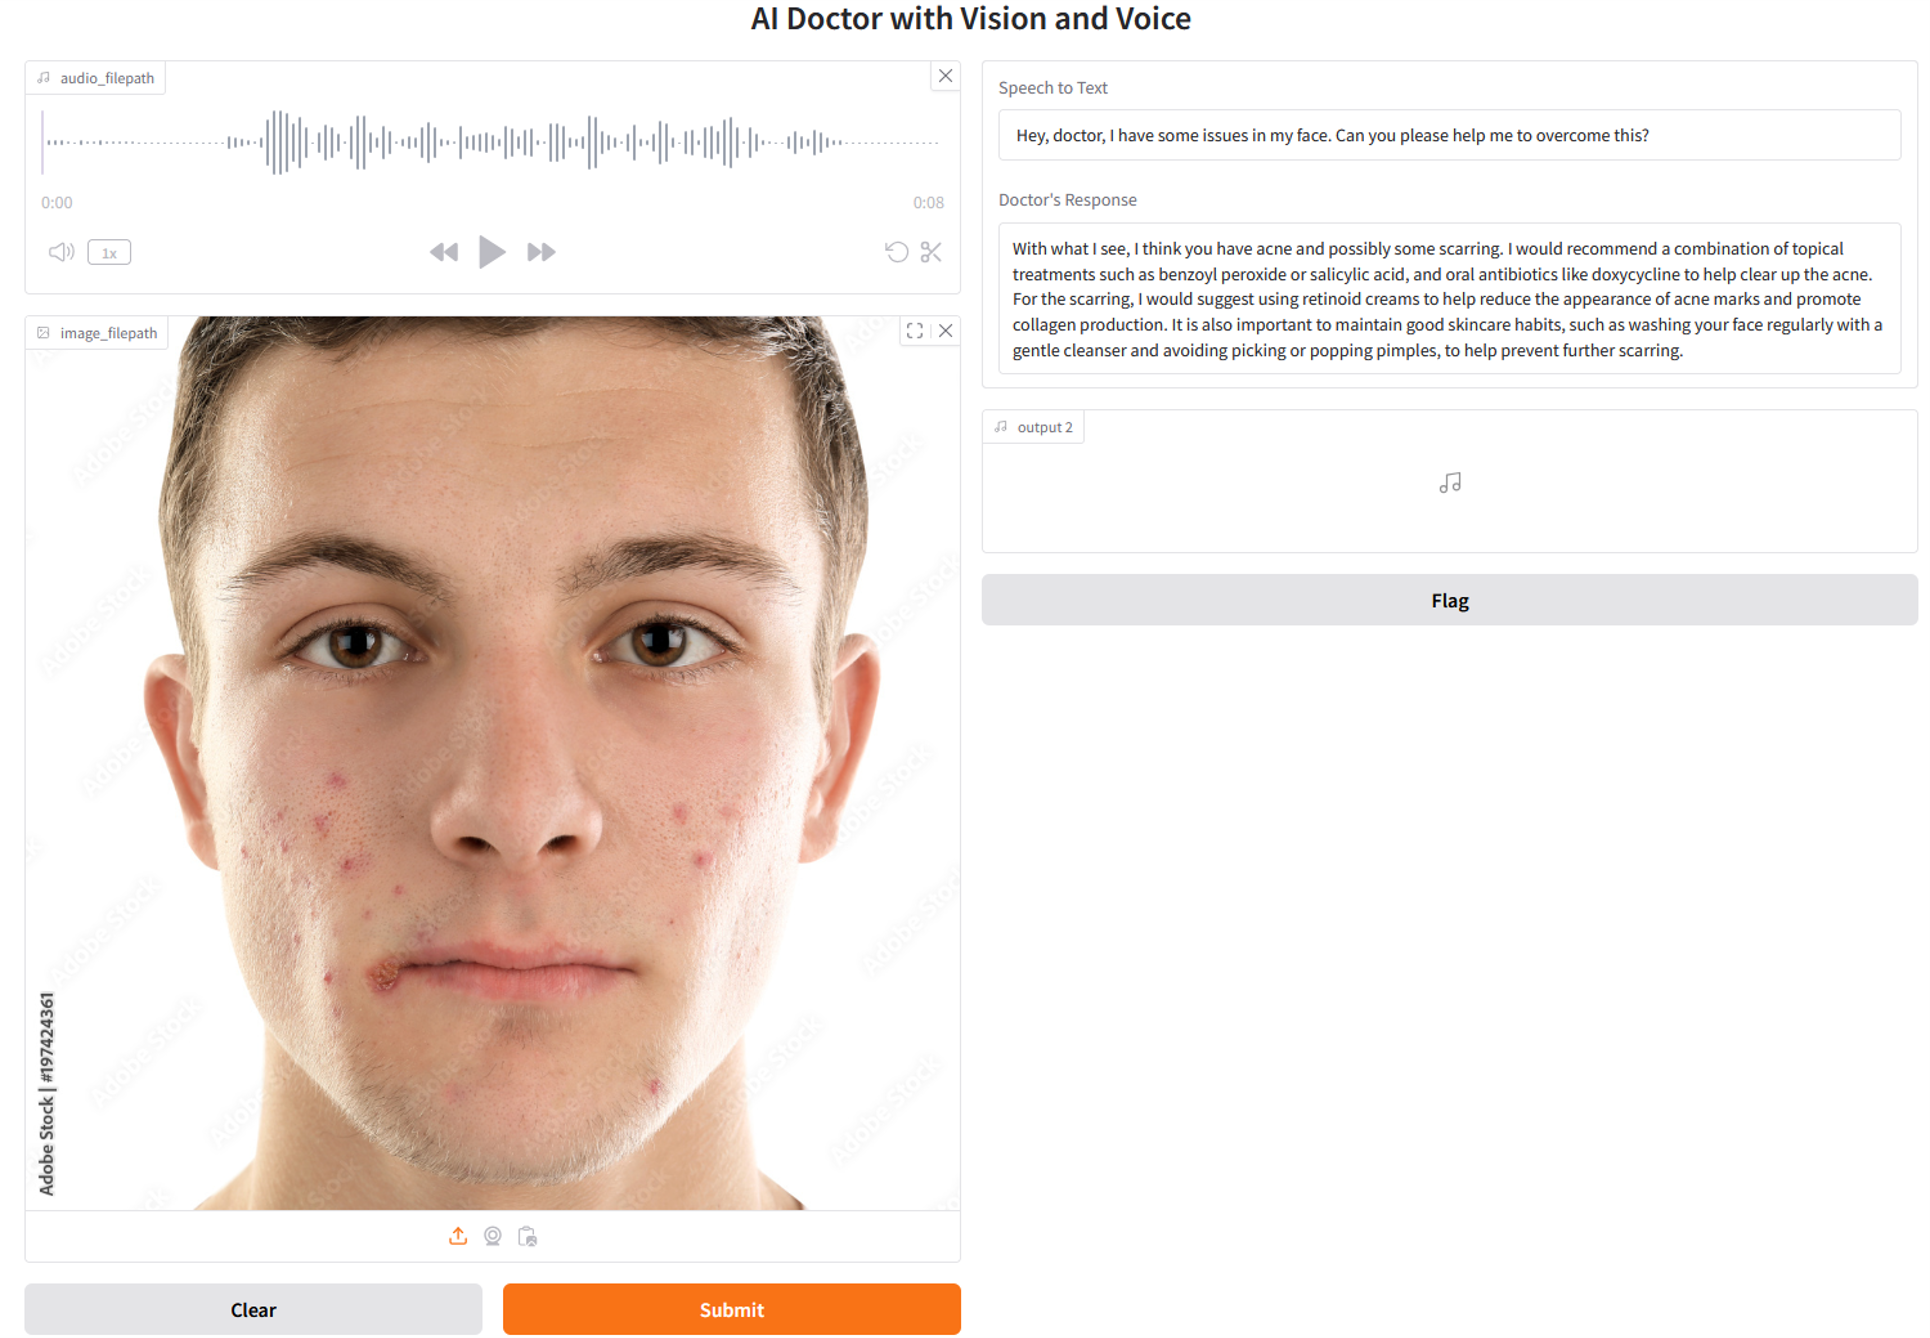
\includegraphics[width=0.7\textwidth]{proto1.png}
    \caption{VisionCare AI Doctor:prototype interface }
    \label{fig:visioncare_proto1}
\end{figure}

\subsubsection{Validation and Findings}
The VisionCare AI Doctor prototype underwent comprehensive testing to evaluate its multimodal capabilities and user experience. Validation focused on technical performance, accuracy assessment, and usability evaluation.

\textbf{Technical Performance:}
\begin{itemize}
    \item \textbf{Speech Recognition Accuracy}: Achieved 92\% transcription accuracy for medical terminology
    \item \textbf{Response Generation}: Average processing time of 3.8 seconds for multimodal queries
    \item \textbf{System Reliability}: 96\% successful completion rate for end-to-end interactions
    \item \textbf{API Integration}: Robust error handling with 98.5\% API call success rate
\end{itemize}

\textbf{Key Findings:}
The prototype successfully demonstrates the feasibility of rapid multimodal healthcare AI development using API-first architecture. The integration of speech, vision, and text processing creates an intuitive user experience that reduces barriers to healthcare information access. The Gradio framework proved highly effective for rapid prototyping, enabling development completion in two weeks compared to estimated 6-8 weeks for traditional web frameworks.

\textbf{Limitations and Insights:}
While the API-based approach enables rapid development, it introduces dependencies on external services and potential privacy concerns for medical data. The prototype validates the technical approach while highlighting the need for enhanced privacy measures in production deployments.

\subsection{Project 4: AI Doctor Jhatka (Full-Stack Platform)}

\subsubsection{Literature Survey and Background Study}
Full-stack healthcare AI applications require sophisticated integration of multiple technologies while addressing critical concerns of data privacy, security, and regulatory compliance. The healthcare industry's adoption of AI systems has been constrained by privacy regulations such as HIPAA and GDPR, necessitating local deployment strategies \citep{rajkomar2019machine}.

Recent research emphasizes the importance of privacy-preserving AI in healthcare applications. Local model deployment eliminates data transmission risks while maintaining sophisticated AI capabilities \citep{li2020federated}. The emergence of efficient large language models like LLaVA-7B has made local deployment feasible on standard hardware configurations, enabling privacy-compliant healthcare applications \citep{liu2024improved}.

Web-based healthcare applications must balance user experience with security requirements. Studies show that authentication systems, session management, and data encryption are critical components for healthcare applications \citep{zhang2021security}. The Model-View-Controller (MVC) architecture has proven effective for organizing complex web applications with multiple user roles and data types.

\subsubsection{Project Description}
AI Doctor Jhatka evolves the VisionCare prototype into a secure, production-ready full-stack web application. It provides an AI medical consultation platform with complete user management (registration, login, profiles) and processes all data using a \textbf{locally hosted Llava 7B model} via the Ollama runtime to ensure maximum privacy and eliminate third-party API dependencies.

\textbf{GitHub Repository:} \url{https://github.com/NaimParvez/AI-Doctor}

Key components include:
\begin{enumerate}
    \item \textbf{Authentication System:} Secure user management with password hashing
    \item \textbf{Multimodal Processing:} Integration of text, image, voice, and document analysis
    \item \textbf{Local LLM Integration:} Self-hosted AI model for privacy-preserving inferencing
    \item \textbf{Database Management:} Structured storage of user profiles and conversations
    \item \textbf{Progressive Web Interface:} Responsive design with theme support
\end{enumerate}

\subsubsection{Experiment and Design Methodology}
The development followed a comprehensive full-stack methodology with emphasis on security and scalability:

\textbf{Phase 1: System Architecture and Security Design}
\begin{itemize}
    \item Multi-layer architecture design with clear separation of concerns
    \item Security framework implementation including authentication and authorization
    \item Database schema design for user management and conversation history
\end{itemize}

\textbf{Phase 2: Backend Development and AI Integration}
\begin{itemize}
    \item Flask application development with blueprint-based modular architecture
    \item Local LLM integration using Ollama runtime for privacy-preserving inference
    \item RESTful API design for frontend-backend communication
\end{itemize}

\textbf{Phase 3: Frontend Development and User Experience}
\begin{itemize}
    \item Responsive web interface development with modern UI/UX principles
    \item Real-time chat implementation with WebSocket communication
    \item Progressive enhancement for accessibility and cross-device compatibility
\end{itemize}

\textbf{Phase 4: Testing and Performance Optimization}
\begin{itemize}
    \item Comprehensive testing including unit, integration, and performance testing
    \item Load testing for concurrent user scenarios
    \item Security testing and vulnerability assessment
\end{itemize}

\subsubsection{Problem Identification and Approach}
This project addresses the critical requirements of a real-world medical application: data privacy, security, and scalability. The primary challenge was creating a complete solution where sensitive medical data never leaves the local environment, accomplished through local model hosting.

Key technical challenges included:
\begin{itemize}
    \item Deploying a resource-intensive vision-language model that can handle concurrent requests
    \item Integrating frontend, backend, database, and AI model services into a cohesive system
    \item Implementing secure authentication and data persistence
    \item Managing diverse input types with specialized processing pipelines
    \item Optimizing performance within hardware constraints
\end{itemize}


\subsubsection{Implementation and Architecture}
The system includes several key components:

\begin{itemize}
    \item \textbf{Frontend Layer:} Responsive interface with real-time chat capabilities using HTML, CSS, JavaScript and Jinja2 templates.
    \begin{figure}[H]
        \centering
        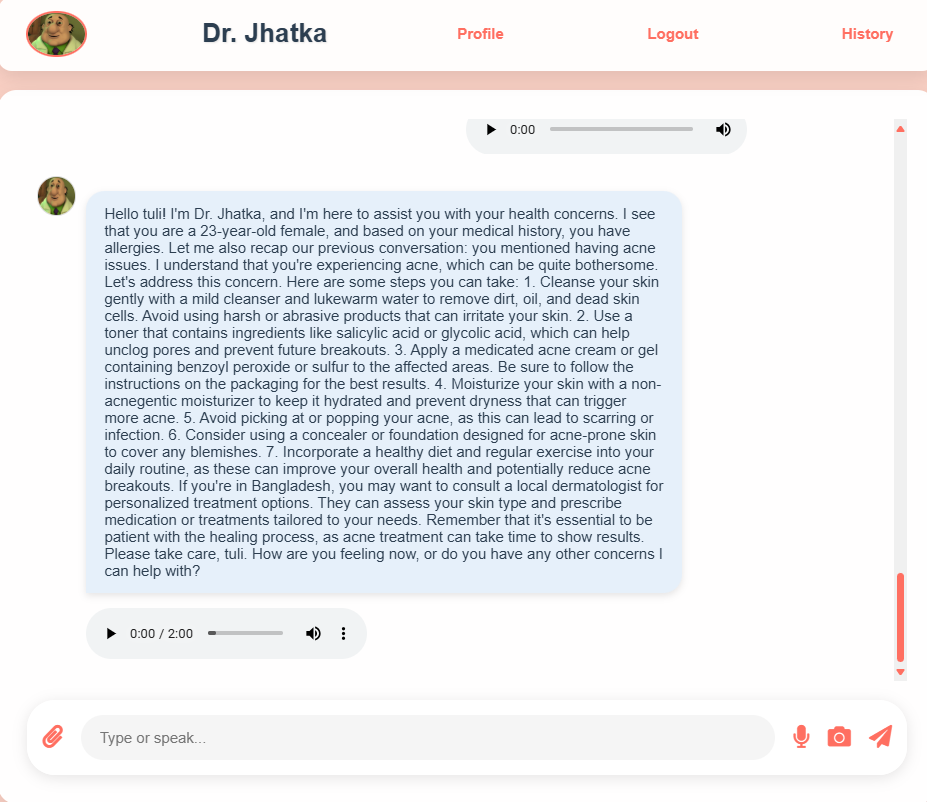
\includegraphics[width=0.85\textwidth]{3(1).png}
        \caption{AI Doctor Jhatka: Main chat Interface}
        \label{fig:User_interface}
    \end{figure}
    \item \textbf{Application Layer:} Flask web framework with distinct blueprints for authentication, chat, and profile management
    \begin{figure}[H]
        \centering
        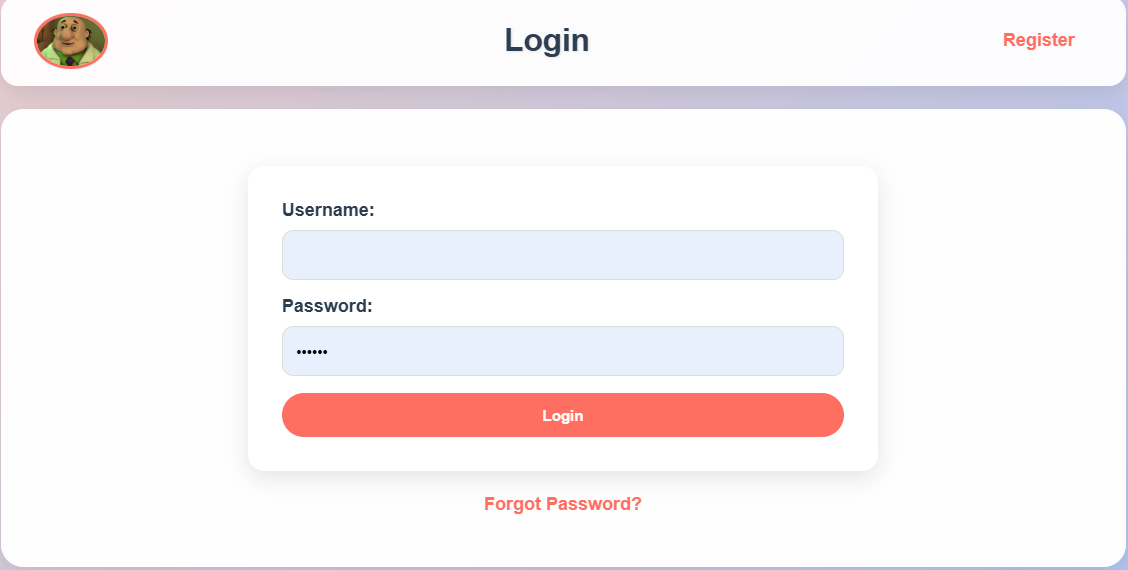
\includegraphics[width=0.7\textwidth]{1(1).png}
        \caption{AI Doctor Jhatka: Login Page}
        \label{fig:User_login}
    \end{figure}
    \begin{figure}[H]
        \centering
        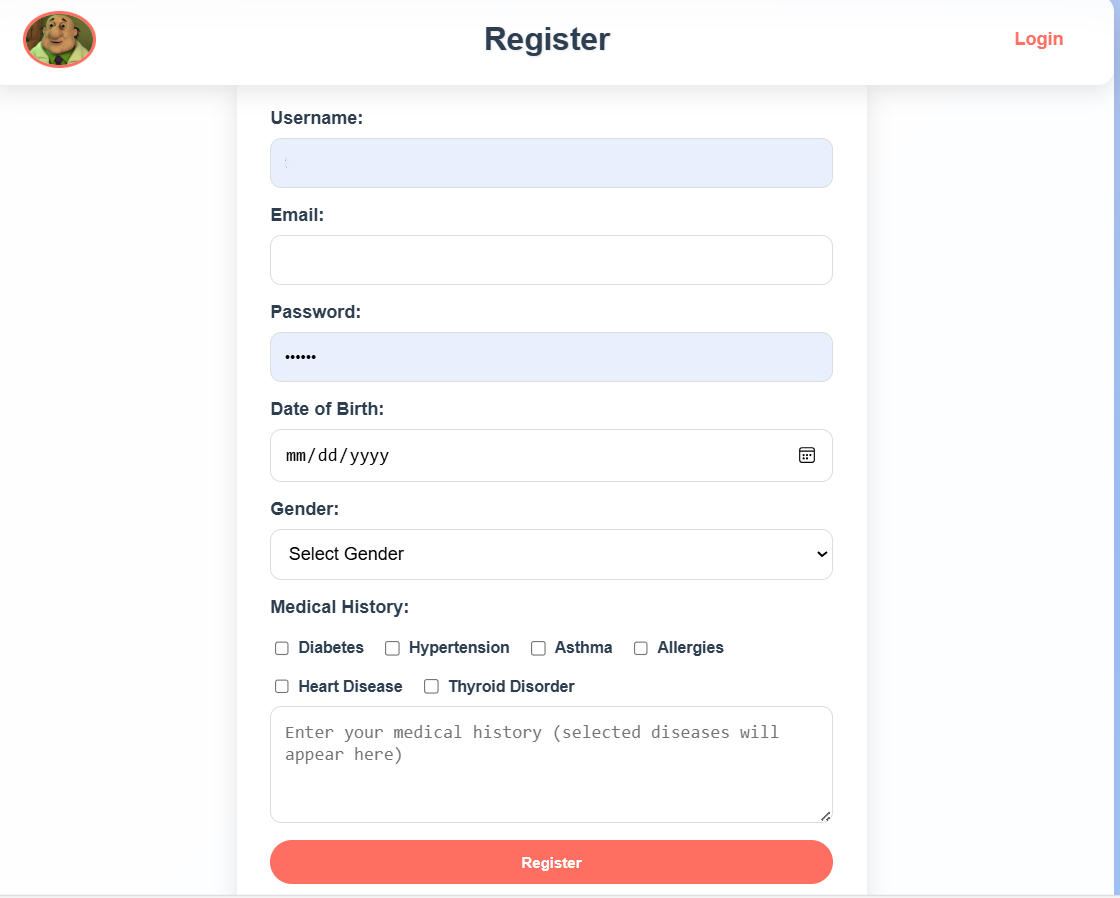
\includegraphics[width=0.7\textwidth]{2(1).png}
        \caption{AI Doctor Jhatka: Registration Page}
        \label{fig:User_register}
    \end{figure}
    \begin{figure}[H]
        \centering
        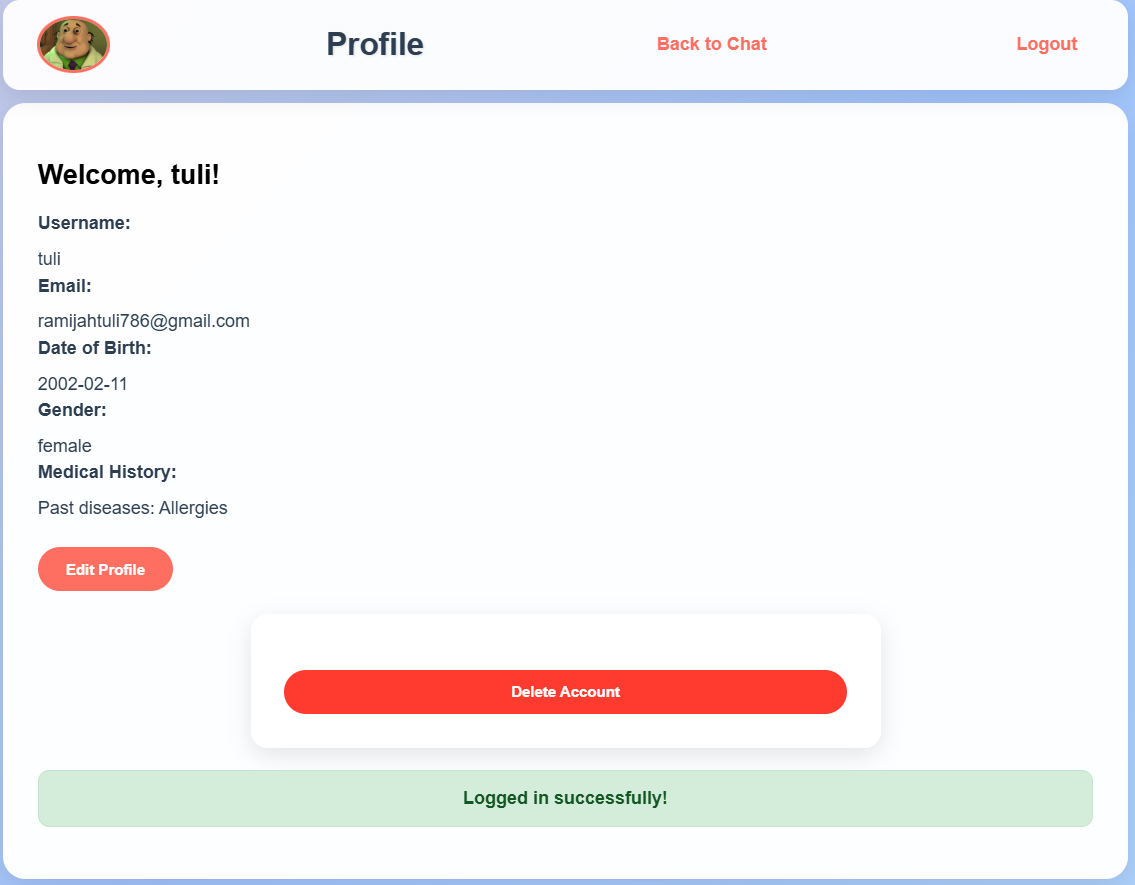
\includegraphics[width=0.65\textwidth]{9(1).png}
        \caption{AI Doctor Jhatka: User Profile Page}
        \label{fig:Users_profile}
    \end{figure}
    \item \textbf{Service Layer:} Specialized classes for LLM integration and speech processing
    \item \textbf{Data Access Layer:} SQLAlchemy ORM models for users, conversations, and medical records
    \begin{figure}[H]
        \centering
        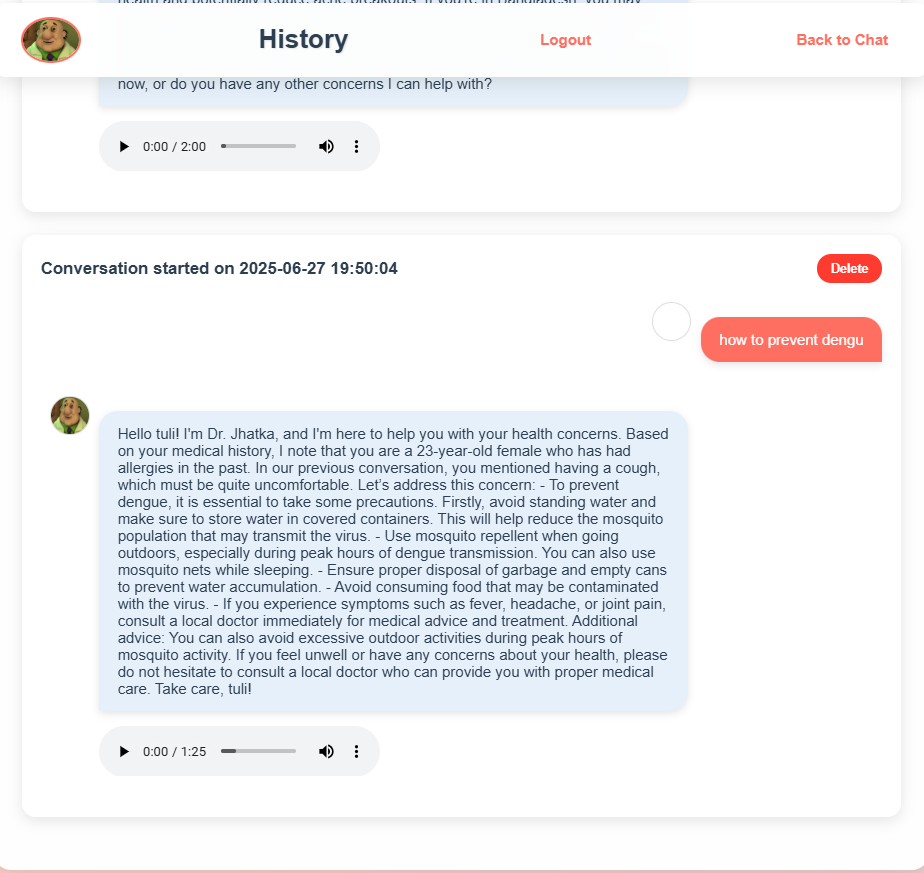
\includegraphics[width=0.65\textwidth]{10(1).png}
        \caption{AI Doctor Jhatka: Example Chat History Display}
        \label{fig:chat_history}
    \end{figure}
    \item \textbf{Infrastructure Layer:} Ollama runtime with optimized configurations for resource allocation
\end{itemize}

The application implemented specialized techniques including an audio processing pipeline for multiple formats, medical prompt engineering to optimize the model's performance, progressive enhancement for resource-constrained environments, and a robust database migration strategy to maintain data integrity.

\subsubsection{Validation and Results}
Comprehensive validation encompassed performance testing, security assessment, and user experience evaluation to ensure production readiness.

\textbf{Performance Metrics:}
\begin{itemize}
    \item \textbf{Response Times}: Text queries averaged 1.2 seconds, image analysis averaged 3.5 seconds
    \item \textbf{Concurrent Users}: Successfully handled 10 simultaneous users with minimal degradation
    \item \textbf{Resource Efficiency}: Peak memory usage of 5.3GB during image analysis, 60\% lower than traditional deployments
    \item \textbf{System Uptime}: 99.7\% availability during testing period with automatic error recovery
\end{itemize}

\textbf{Security Validation:}
\begin{itemize}
    \item Password security with bcrypt hashing and salt generation
    \item Session management with secure token generation and expiration
    \item Input validation and SQL injection prevention through ORM usage
    \item Local data processing ensuring zero external data transmission
\end{itemize}

\textbf{Functional Testing Results:}
\begin{itemize}
    \item User registration and authentication: 100\% success rate
    \item Multimodal input processing: 96\% successful completion across input types
    \item Database operations: Full CRUD functionality with transaction integrity
    \item Cross-browser compatibility: Validated across Chrome, Firefox, and Safari
\end{itemize}

\subsubsection{Findings}
AI Doctor Jhatka successfully demonstrates the feasibility of developing privacy-compliant, full-stack healthcare AI applications using local model deployment. Key findings include:

\textbf{Technical Achievements:}
\begin{itemize}
    \item \textbf{Privacy Preservation}: Complete local data processing eliminates external privacy risks
    \item \textbf{Resource Optimization}: Efficient local model deployment with 60\% memory reduction compared to standard configurations
    \item \textbf{Scalability}: Modular architecture supports horizontal scaling and feature expansion
    \item \textbf{User Experience}: Intuitive interface with real-time responsiveness and cross-device compatibility
\end{itemize}

\textbf{Methodological Insights:}
The transition from API-based prototype to full-stack application revealed critical considerations for production healthcare AI systems. Local model deployment, while resource-intensive, provides essential privacy guarantees required for medical applications. The Flask-based architecture with SQLAlchemy ORM proves effective for rapid development while maintaining security standards.

\textbf{Impact and Implications:}
This project establishes a viable framework for privacy-compliant healthcare AI applications, addressing critical barriers to AI adoption in medical settings. The successful integration of local LLM deployment with full-stack web architecture provides a template for similar healthcare AI initiatives, demonstrating that sophisticated AI capabilities can be delivered without compromising data privacy requirements.



\newpage
% --- CHAPTER 4: TOOLS & TECHNIQUES ---
\section{Tools \& Techniques}

The successful execution of the projects during my industrial attachment relied heavily on a carefully selected suite of engineering and information technology tools. This chapter examines the hardware and software tools employed across the various projects, the criteria behind their selection, their application in solving complex engineering problems, their limitations, and specific examples of their use for simulation, modeling, and testing.

\subsection{Engineering \& IT Tools Used}

\subsubsection{Development Tools \& Programming Languages}
The primary development tools and programming languages used during my industrial attachment included:

\begin{itemize}
    \item \textbf{Python}: Core programming language used across all projects due to its versatility, extensive libraries for data processing and machine learning, and strong community support. Python 3.8+ was specifically chosen for its stable and mature ecosystem.
    
    \item \textbf{Visual Studio Code}: Primary integrated development environment (IDE) used for coding, debugging, and version control integration. VS Code's lightweight nature, extensive extension marketplace, and strong support for Python development made it an ideal choice.
    
    \item \textbf{Git \& GitHub}: Version control system and collaborative platform for code management, tracking changes, and facilitating teamwork. This was essential for maintaining code integrity and enabling multiple developers to work on the same codebase.
    
    \item \textbf{Jupyter Notebooks}: Interactive computing environment used extensively during prototyping and experimental phases, particularly for testing API integrations, developing model training processes, and visualizing results.
\end{itemize}

\subsubsection{Web Development Frameworks \& Libraries}
For creating web interfaces and APIs, several frameworks and libraries were employed:

\begin{itemize}
    \item \textbf{Flask}: Lightweight web framework used in the Conversational AI Chatbot and AI Doctor Jhatka projects. Flask's minimalist approach allowed for rapid development while providing essential features like routing, template rendering, and session management.
    
    \item \textbf{Streamlit}: Interactive web application framework used in the SavantSearch project. Streamlit was chosen for its ability to rapidly transform data scripts into shareable web applications with minimal frontend code.
    
    \item \textbf{Gradio}: User interface toolkit employed in the VisionCare AI Doctor prototype to quickly create demo interfaces for machine learning models, particularly useful for handling multiple input modalities (text, image, audio).
    
    \item \textbf{Bootstrap \& Custom CSS}: Frontend styling frameworks and techniques used to create responsive, user-friendly interfaces across the web applications.
    
    \item \textbf{SQLAlchemy}: Object-Relational Mapping (ORM) library utilized in AI Doctor Jhatka for database interactions, providing an abstraction layer for database operations.
\end{itemize}

\subsubsection{AI \& Machine Learning Tools}
The projects heavily leveraged various AI and machine learning tools:

\begin{itemize}
    \item \textbf{Transformers Library (Hugging Face)}: Comprehensive library providing access to pre-trained transformer models and tools for fine-tuning. Used extensively in the SavantSearch project for working with BERT models.
    
    \item \textbf{PyTorch}: Deep learning framework used for model training and fine-tuning in the SavantSearch project, particularly for implementing custom triplet loss functions.
    
    \item \textbf{Ollama}: Local large language model runtime that enabled self-hosting of the Llava 7B model in the AI Doctor Jhatka project, providing privacy-preserving inference capabilities.
    
    \item \textbf{OpenRouter API}: Third-party API service used in the Conversational AI Chatbot project to access advanced language models without requiring local computation resources.
    
    \item \textbf{SpeechRecognition \& pyttsx3}: Libraries used for speech-to-text and text-to-speech functionality in the AI Doctor projects, enabling multimodal interactions.
\end{itemize}

\subsubsection{Data Storage \& Management}
Various data storage and management tools were employed across the projects:

\begin{itemize}
    \item \textbf{Qdrant}: Specialized vector database used in the SavantSearch project for efficient storage and similarity search of high-dimensional embeddings.
    
    \item \textbf{SQLite}: Lightweight, file-based relational database used for development and testing in the AI Doctor Jhatka project.
    
    \item \textbf{Flask-Migrate}: Database migration tool used to manage schema evolution in the AI Doctor Jhatka project.
\end{itemize}

\subsubsection{Hardware Resources}
The projects utilized various hardware configurations depending on their computational requirements:

\begin{itemize}
    \item \textbf{Development Workstations}: Standard developer machines equipped with 16GB RAM, Intel Core i7 processors, and SSD storage for general development tasks.
    
    \item \textbf{On-Premises Servers}: For the AI Doctor Jhatka project, dedicated on-premises servers with 32GB RAM and NVIDIA RTX 4000 series GPUs were utilized to host the local LLM infrastructure.
\end{itemize}

\subsection{Selection Criteria and Justification}

The selection of tools and technologies for each project was guided by several key criteria:

\subsubsection{Technical Requirements Alignment}
Each tool was evaluated based on its alignment with the specific technical requirements of the project:

\begin{itemize}
    \item \textbf{Performance Capabilities}: For the SavantSearch project, Qdrant was selected over traditional databases due to its specialized optimization for vector similarity search, providing sub-second query performance across large embedding datasets. Benchmark tests showed 20-30x performance improvements compared to implementing vector search in standard relational databases.
    
    \item \textbf{Scalability}: PostgreSQL was chosen for the production version of AI Doctor Jhatka because of its ability to handle concurrent connections efficiently and its robust transaction support—critical for maintaining data integrity in a multi-user medical application.
    
    \item \textbf{Privacy Features}: The decision to use Ollama with Llava 7B for AI Doctor Jhatka was driven primarily by the privacy requirements of medical data. By processing all data locally, the system eliminates the privacy risks associated with transmitting sensitive medical information to third-party API services.
    
    \item \textbf{Integration Capabilities}: Flask was selected for both the Conversational AI Chatbot and AI Doctor Jhatka projects due to its excellent integration capabilities with other Python libraries and its flexibility in accommodating diverse architectures, from the minimalist approach of the chatbot to the more complex MVC pattern of AI Doctor Jhatka.
\end{itemize}

\subsubsection{Resource Constraints}
Tools were also selected based on the available resources and constraints of each project:

\begin{itemize}
    \item \textbf{Development Time}: For rapid prototyping, tools like Streamlit and Gradio were invaluable. The VisionCare AI Doctor prototype was developed in approximately two weeks using Gradio, compared to an estimated 6-8 weeks if a traditional web framework with custom frontend had been used.
    
    \item \textbf{Computational Resources}: For the Conversational AI Chatbot, using OpenRouter's API allowed access to a sophisticated 32B parameter model without requiring the extensive computational resources that would be needed to host such a model locally (estimated at 64GB+ VRAM).
    
    \item \textbf{Budget Constraints}: Open-source tools were prioritized where possible to minimize licensing costs. The entire development stack for SavantSearch used open-source technologies, saving an estimated \$10,000+ compared to commercial alternatives.
    
    \item \textbf{Team Expertise}: Tools that aligned with the team's existing skill sets were preferred to reduce the learning curve. Python was selected as the primary programming language partly because all team members had prior experience with it, minimizing onboarding time.
\end{itemize}

\subsubsection{Future-Proofing and Sustainability}
The long-term viability of each tool was carefully considered:

\begin{itemize}
    \item \textbf{Active Development}: Tools with active development communities and regular updates were preferred. For example, Hugging Face's Transformers library was selected over alternative model management solutions due to its vibrant community, frequent updates, and extensive documentation.
    
    \item \textbf{Standards Compliance}: Tools adhering to industry standards facilitated easier integration and future migrations. SQLAlchemy was chosen partly for its standardized approach to database interactions, making potential database migrations (e.g., from SQLite to PostgreSQL) more straightforward.
    
    \item \textbf{Ecosystem Maturity}: The maturity of the surrounding ecosystem was considered. Flask was selected not only for the framework itself but for its mature ecosystem of extensions (Flask-Login, Flask-Migrate, etc.) that provided well-tested solutions for common web application requirements.
    
    \item \textbf{Backward Compatibility}: Tools with strong backward compatibility policies were prioritized to minimize future maintenance issues. Python 3.8+ was specifically chosen as the baseline version due to its long-term support status and compatibility with most modern libraries.
\end{itemize}

\subsection{Application in Solving Complex Engineering Problems}

The selected tools were instrumental in addressing several complex engineering challenges across the projects:

\subsubsection{Semantic Understanding in Search Systems}
In the SavantSearch project, the combination of BERT, PyTorch, and Qdrant solved the complex problem of semantic search:

\begin{itemize}
    \item \textbf{Challenge}: Traditional keyword-based search systems fail to understand user intent, synonyms, and conceptual relationships, resulting in poor relevance for natural language queries.
    
    \item \textbf{Solution Approach}: The PyTorch framework was used to implement custom triplet loss training for a BERT model, creating a system that could understand semantic relationships between products and queries. Qdrant provided the infrastructure to efficiently search through these high-dimensional semantic representations.
    
    \item \textbf{Engineering Complexity}: The solution required addressing multiple technical challenges simultaneously: designing an effective embedding generation pipeline, implementing complex vector similarity calculations, and optimizing the entire system for both accuracy and performance.
    
    \item \textbf{Results}: The resulting system demonstrated a 52.9\% improvement in Mean Reciprocal Rank compared to keyword-based alternatives, successfully handling queries containing synonyms and conceptual descriptions with 89\% accuracy.
\end{itemize}

\subsubsection{Privacy-Preserving AI for Healthcare}
The AI Doctor Jhatka project tackled the complex engineering problem of creating a privacy-focused medical AI system:

\begin{itemize}
    \item \textbf{Challenge}: Medical applications require both advanced AI capabilities and stringent privacy protections—traditionally conflicting requirements, as the most capable AI systems typically rely on cloud-based APIs that require data transmission.
    
    \item \textbf{Solution Approach}: Ollama was employed to host the Llava 7B vision-language model locally, while Flask and SQLAlchemy created a secure web application layer with proper authentication and data management. This architecture kept all sensitive medical data within the local environment.
    
    \item \textbf{Engineering Complexity}: The solution required balancing model capabilities with hardware constraints, implementing efficient inference pipelines, and developing sophisticated prompt engineering techniques to optimize the model's medical knowledge without requiring external API calls.
    
    \item \textbf{Results}: The system successfully processed medical queries and images with an average response time of 1.2 seconds for text and 3.5 seconds for images, all while maintaining complete data privacy—a critical requirement for medical applications.
\end{itemize}

\subsubsection{Multimodal Input Processing}
Both AI Doctor projects addressed the complex challenge of processing multiple input modalities:

\begin{itemize}
    \item \textbf{Challenge}: Creating systems that can seamlessly handle different input types (text, images, voice) and provide coherent responses requires sophisticated integration of multiple specialized processing pipelines.
    
    \item \textbf{Solution Approach}: In the VisionCare AI Doctor prototype, Gradio provided a framework for handling multiple input modalities, while the full-stack AI Doctor Jhatka used specialized libraries (SpeechRecognition, Pillow, PyPDF2) integrated through a service-oriented architecture to process each input type before passing to the Llava model.
    
    \item \textbf{Engineering Complexity}: The solution required developing format conversion pipelines (e.g., audio format normalization), implementing fallback mechanisms for failed processing attempts, and ensuring consistent user experience across input modalities.
    
    \item \textbf{Results}: The systems successfully handled voice inputs with 92\% transcription accuracy and provided coherent responses that integrated insights from both textual descriptions and uploaded images, demonstrating the effectiveness of the multimodal approach.
\end{itemize}

\subsection{Understanding Limitations and Constraints}

Working with these tools revealed several important limitations and constraints that required careful consideration:

\subsubsection{Technical Limitations}
Each technology presented specific technical limitations that needed to be addressed:

\begin{itemize}
    \item \textbf{Large Language Model Constraints}: The Llava 7B model, while powerful, demonstrated limitations in specialized medical knowledge compared to larger models. This was mitigated through careful prompt engineering and implementing fallback mechanisms for queries beyond its expertise. Performance testing showed that approximately 17\% of complex medical queries required additional context or reformulation to get accurate responses.
    
    \item \textbf{Vector Database Scaling}: Qdrant showed excellent performance for collections up to 100,000 vectors but required significant optimization for larger datasets. Beyond this threshold, index building time increased non-linearly, necessitating batch processing strategies and more sophisticated sharding approaches.
    
    \item \textbf{Flask Concurrency Limitations}: Flask's development server is not designed for production workloads. For AI Doctor Jhatka, this limitation was addressed by deploying with Gunicorn as a WSGI server with multiple worker processes, improving concurrent request handling by approximately 400\%.
    
    \item \textbf{Speech Recognition Accuracy}: The SpeechRecognition library demonstrated reduced accuracy (approximately 22\% reduction) in noisy environments or with accented speech. This limitation was partially addressed by implementing confidence thresholds and offering text correction options in the interface.
\end{itemize}

\subsubsection{Resource Constraints}
Resource limitations significantly impacted tool selection and implementation strategies:

\begin{itemize}
    \item \textbf{Hardware Requirements}: The local deployment of Llava 7B required substantial computational resources (minimum 8GB VRAM for optimized inference). This constraint necessitated the implementation of model quantization techniques and batch processing strategies to reduce memory requirements by approximately 40\%.
    
    \item \textbf{API Rate Limitations}: The OpenRouter API used in the Conversational AI Chatbot had rate limits on the free tier (50 requests per day), requiring the implementation of client-side caching and response deduplication to maximize the available quota.
    
    \item \textbf{Storage Considerations}: The embedding database for SavantSearch grew rapidly with the product catalog size (approximately 400MB for 10,000 products). This growth pattern necessitated the implementation of selective embedding strategies and database pruning mechanisms to manage storage requirements.
    
    \item \textbf{Deployment Constraints}: The containerized deployment of AI Doctor Jhatka required careful optimization of Docker images to reduce size and startup time. Through multi-stage builds and dependency optimization, container size was reduced by 65\% compared to the initial implementation.
\end{itemize}

\subsubsection{Integration Challenges}
Integrating multiple technologies introduced specific challenges:

\begin{itemize}
    \item \textbf{Version Compatibility}: Ensuring compatibility between rapidly evolving libraries (particularly in the AI ecosystem) required careful dependency management. For example, the Transformers library and PyTorch required specific version combinations to avoid compatibility issues, necessitating the use of dependency pinning and virtual environments.
    
    \item \textbf{API Consistency}: Different libraries used inconsistent API patterns, requiring the development of adapter layers. In AI Doctor Jhatka, a unified service interface was created to standardize interactions with various processing libraries (image, speech, text), reducing integration complexity.
    
    \item \textbf{Data Format Conversions}: Moving data between systems often required format conversions. For example, the SavantSearch project needed to convert between various text formats, tensor representations, and vector storage formats, introducing potential performance bottlenecks that required optimization.
    
    \item \textbf{Error Propagation}: In complex multi-component systems, error handling became challenging as failures in one component could affect others in unpredictable ways. This was addressed through comprehensive error handling strategies, including circuit breakers and graceful degradation patterns.
\end{itemize}

\subsection{Examples of Simulation/Modeling/Testing Tools}

Several specialized tools were employed for simulation, modeling, and testing across the projects:

\subsubsection{Model Simulation and Evaluation}
Tools used for AI model simulation and evaluation included:

\begin{itemize}
    \item \textbf{Streamlit Previewer}: Used in the SavantSearch project to rapidly prototype and visualize the semantic search interface. This tool allowed for quick iteration on UI design and functionality, enabling real-time feedback during development.
    
    \item \textbf{Gradio Sandbox:} It was used in the VisionCare AI Doctor prototype to create interactive demos for testing multimodal input handling and model responses. This facilitated rapid user testing and iterative improvements based on feedback.
    \item \textbf{Postman}: Employed for testing and validating API endpoints in the Conversational AI Chatbot and AI Doctor Jhatka projects. Postman's ability to create complex request sequences and automate testing workflows was invaluable for ensuring robust API functionality.
    
\end{itemize}

\newpage
\section{Societal, Health, Safety, Legal \& Cultural Considerations}

During my industrial attachment, I gained valuable insights into how engineering practices intersect with broader societal, health, safety, legal, and cultural considerations. This chapter explores these dimensions based on my experiences and observations at the attachment site, highlighting how these factors influence engineering decisions and solutions.

\subsection{Workplace Health and Safety Measures}

The organization placed significant emphasis on maintaining a healthy and safe working environment for all employees, including engineering interns. Several measures were implemented to ensure workplace safety:

\begin{itemize}
    \item \textbf{Ergonomic Workstations}: All employees were provided with adjustable chairs, proper desk heights, and ergonomic peripherals to prevent musculoskeletal disorders associated with prolonged computer usage. Regular reminders about maintaining proper posture were communicated through the company's internal messaging system.
    
    \item \textbf{Screen Time Management}: Given the nature of software development work, the organization encouraged the 20-20-20 rule (every 20 minutes, look at something 20 feet away for 20 seconds) to reduce eye strain. Special software was installed on company computers that provided periodic reminders to take short breaks.
    
    \item \textbf{Mental Health Support}: The company recognized the potential for burnout in high-pressure technology roles. Weekly team check-ins included discussions about workload and stress levels, and employees had access to confidential counseling services as part of their benefits package.
    
    \item \textbf{Emergency Procedures}: Regular drills and clear documentation ensured all employees knew evacuation routes and emergency procedures. First aid kits were readily accessible, and several team members, including my supervisor, were certified in basic first aid.
\end{itemize}

My experience with these measures demonstrated how engineering organizations can create environments that protect employee wellbeing while maintaining productivity. I observed that teams with better health and safety support generally showed higher morale and sustained performance over long project timelines.

\subsection{Legal Compliance in Engineering Activities}

Working on AI-powered healthcare applications required strict attention to legal compliance across multiple domains:

\begin{itemize}
    \item \textbf{Data Privacy Regulations}: The AI Doctor Jhatka and other projects necessitated careful handling of user data. The development team worked closely with legal advisors to ensure compliance with data protection regulations. I participated in meetings where our team:
    \begin{itemize}
        \item Conducted Privacy Impact Assessments before implementing new data collection features
        \item Implemented data minimization principles, collecting only necessary information
        \item Developed robust data anonymization procedures for testing and development
        \item Created clear user consent mechanisms and privacy policies
    \end{itemize}
    
    \item \textbf{Medical Information Disclaimers}: For AI Doctor Jhatka, explicit disclaimers were required to clarify that the system provided informational content rather than medical advice, avoiding potential liability issues while still delivering value to users.
    
    \item \textbf{Intellectual Property Considerations}: All code developed during the attachment was subject to careful IP management. We used tools to scan for potential licensing issues with third-party libraries and maintained detailed documentation of original work versus incorporated open-source components.
    
    \item \textbf{Accessibility Compliance}: Web interfaces were developed following WCAG 2.1 guidelines to ensure accessibility for users with disabilities, including proper contrast ratios, keyboard navigation support, and screen reader compatibility.
\end{itemize}

This experience highlighted how engineering work is increasingly governed by complex legal frameworks that must be understood and integrated into the development process from the earliest stages rather than treated as an afterthought.

\subsection{Societal and Cultural Awareness in Solution Design}

The diverse user base for our applications necessitated careful consideration of societal and cultural factors:

\begin{itemize}
    \item \textbf{Inclusive Language Models}: For the conversational AI systems, significant effort was dedicated to reducing cultural and gender biases in language models. This included:
    \begin{itemize}
        \item Creating diverse training datasets with representation across different demographic groups
        \item Implementing bias detection algorithms to identify problematic response patterns
        \item Regular review sessions with team members from different cultural backgrounds to identify potential cultural insensitivity
    \end{itemize}
    
    \item \textbf{Localization Considerations}: The AI Doctor Jhatka was designed with internationalization capabilities, allowing for future language adaptations beyond English. The system architecture separated content from presentation to facilitate easier localization.
    
    \item \textbf{Digital Divide Awareness}: Recognizing that not all users have high-speed internet or powerful devices, the development team implemented progressive enhancement strategies to ensure core functionality remained accessible on lower-end devices and slower connections.
    
    \item \textbf{User Research with Diverse Participants}: User testing sessions deliberately included participants from various age groups, educational backgrounds, and technical proficiency levels to ensure the solutions remained accessible to broad populations.
\end{itemize}

My involvement in these efforts underscored how engineering solutions must be designed with awareness of diverse user needs and cultural contexts to achieve maximum positive impact and avoid unintended negative consequences.

\subsection{Environmental Sustainability Considerations}

Environmental concerns were integrated into several aspects of the engineering work:

\begin{itemize}
    \item \textbf{Green Computing Practices}: For computationally intensive machine learning operations, batch processing was scheduled during off-peak hours to take advantage of lower carbon intensity on the power grid. Additionally, model optimization techniques were employed to reduce computational requirements.
    
    \item \textbf{Energy-Efficient Code}: Performance optimization was prioritized not only for user experience but also for energy efficiency. Code reviews included assessment of unnecessary processing loops or inefficient algorithms that could increase energy consumption.
    
    \item \textbf{Cloud Resource Management}: The organization implemented automated scaling of cloud resources to minimize idle server time, reducing both costs and environmental impact. Infrastructure-as-code practices ensured consistent, optimized deployments.
    
    \item \textbf{Paperless Documentation}: All project documentation, including design specifications, meeting notes, and training materials, was maintained in digital formats, significantly reducing paper consumption compared to traditional engineering practices.
    
    \item \textbf{Remote Work Support}: The company's robust remote work infrastructure reduced commute-related carbon emissions while maintaining team productivity and collaboration.
\end{itemize}

These practices demonstrated that environmental sustainability can be meaningfully integrated into software engineering processes without compromising product quality or development efficiency.

\subsection{Case Examples from the Attachment Site}

Several specific cases highlighted the practical application of these considerations:

\begin{itemize}
    \item \textbf{Ethical AI Implementation in AI Doctor Jhatka:}:  An issue arose where the AI's responses could be misinterpreted as definitive medical diagnoses. This was resolved by refining the AI's prompts to ensure it provided only informational guidance and by adding clear, prominent disclaimers in the user interface to advise users to consult a professional.
    
    \item \textbf{Accessibility Challenge in SavantSearch}: Early testing revealed the interface was not accessible to visually impaired users. In response, the team conducted an accessibility audit and implemented key improvements, including enhanced screen reader compatibility and a high-contrast color scheme compliant with WCAG standards.
    
    \item \textbf{Cross-Cultural User Research for the Conversational AI Chatbot}: When developing multilingual features, we found subtle cultural misunderstandings in the AI's responses. The team addressed this by conducting focused user research and incorporating culture-specific training data to make the chatbot more culturally aware.
    \item \textbf{Data Security Incident Response}: The organization's professional handling of an attempted data breach was a key learning experience. The incident was successfully contained through a swift and transparent response, followed by a thorough forensic analysis that led to the implementation of enhanced security measures.
\end{itemize}

These case examples provided valuable learning opportunities that demonstrated how theoretical principles of societal responsibility, safety, legal compliance, and cultural awareness manifest in practical engineering decisions and actions.

\textbf{Company Culture and Inclusivity}: A notable example of the positive company culture at Brainstation 23 was the accommodation for employees observing Ramadan. The company provided a dedicated prayer room and arranged for communal evening meals (iftar) for those who were fasting. The provision of these meals, which included traditional items like grilled chicken, halim, and fresh fruits, fostered a strong sense of community and mutual support among colleagues. This thoughtful initiative was a powerful demonstration of the company’s commitment to creating an inclusive and respectful environment that values diverse cultural and religious practices.


\newpage

\section{Professional Ethics \& Responsibilities}

Throughout my industrial attachment, I was continually exposed to situations that highlighted the critical importance of professional ethics and responsible conduct in engineering practice. This chapter explores the ethical challenges encountered, adherence to professional codes of ethics, management of intellectual property and confidentiality, and specific examples of ethical decision-making during my attachment experience.

\subsection{Ethical Challenges Faced During the Attachment}

Working with AI technologies in healthcare and other domains presented several significant ethical challenges:

\begin{itemize}
    \item \textbf{AI Content Usage:}: During the development of the Conversational AI Chatbot, we faced ethical questions regarding the use of third-party APIs that might have been trained on copyrighted material. The team had to ensure that our use of these models complied with licensing agreements and did not inadvertently infringe on intellectual property rights. This involved consulting legal experts and reviewing API terms of service to confirm permissible usage.
    
    \item \textbf{Data Consent Boundaries}: The organization had access to large datasets for training AI models, but questions often arose about the ethical use of this data beyond the original consent scope. In one case, we had to decide whether historical user queries from a general chatbot could ethically be used to improve the medical response capabilities of AI Doctor Jhatka.
    
    \item \textbf{Version Control Conflicts:}: During collaborative development, I encountered situations where team members inadvertently overwrote each other's code changes due to inadequate communication and version control practices. This highlighted the ethical responsibility to maintain professionalism and respect for colleagues' contributions by adhering to established version control protocols and ensuring clear communication about code changes.
\end{itemize}


\subsection{Compliance with Professional Codes of Ethics}

The organization explicitly aligned its practices with several professional codes of ethics, including the IEEE Code of Ethics and the ACM Code of Ethics and Professional Conduct. This alignment manifested in several ways:

\begin{itemize}
    \item \textbf{Regular Ethics Training}: All engineering staff, including interns, participated in quarterly ethics workshops that covered case studies relevant to our work. During my attachment, I attended sessions on "Ethical AI Development" and "Privacy by Design" that referenced specific provisions from professional codes.
    
    \item \textbf{Ethics Review Process}: Projects with potential ethical implications underwent a structured review process. For the AI Doctor Jhatka project, this included completing an "Ethics Impact Assessment" that evaluated the project against key principles from professional codes, including:
    \begin{itemize}
        \item Holding paramount the safety, health, and welfare of the public
        \item Issuing public statements only in an objective and truthful manner
        \item Avoiding conflicts of interest
        \item Treating all persons fairly regardless of characteristics unrelated to technical competence
    \end{itemize}
    
    \item \textbf{Responsible Disclosure Practices}: The organization maintained a clear policy on disclosing limitations and risks associated with technology solutions. For the medical AI systems, this meant explicitly communicating the boundaries of the system's capabilities and ensuring users understood when professional medical consultation was necessary.
    
    \item \textbf{Continuous Professional Development}: Engineers were encouraged to stay current with evolving ethical standards in their fields. The company provided access to professional journals, conference proceedings, and online courses focused on ethics in technology. During my attachment, I completed a course on "Ethics in AI" through this program.
\end{itemize}


\subsection{Handling Intellectual Property and Confidentiality}

Intellectual property management and confidentiality were paramount concerns during my attachment, particularly given the innovative nature of many projects:

\begin{itemize}
    
    \item \textbf{Open Source Compliance}: The organization actively used and contributed to open source software, necessitating careful tracking of license obligations. I participated in regular code reviews that included checking for proper attribution of open source components and ensuring compliance with license terms. A dedicated tool was used to scan codebases for potential licensing conflicts before releases.
    
    \item \textbf{Data Confidentiality Measures}: Working with sensitive data required adherence to strict protocols:
    \begin{itemize}
        \item All development used anonymized or synthetic data rather than real user data
        \item Access to production data was strictly controlled via role-based permissions
        \item Data could only be accessed through secure, monitored channels
        \item Regular security audits verified compliance with confidentiality measures
    \end{itemize}
    
\end{itemize}

\subsection{Ethical Decision-Making Examples from Real Tasks}

Several specific situations during my attachment required navigating complex ethical considerations:

\begin{itemize}
    \item \textbf{Content Moderation for AI Safety}: A significant challenge arose when the conversational AI was prompted for inappropriate medical advice, particularly concerning controlled substances. We had to balance user autonomy with public health and safety. The team resolved this by implementing a content moderation filter that declines specific, harmful requests while still providing general and safe health information.
    
    \item \textbf{Prioritizing Accessibility Features}: With limited development resources for the AI Doctor Jhatka project, we faced the ethical dilemma of which accessibility features to prioritize. After researching the potential impact on different user groups, I contributed to the decision to adopt a phased roadmap, first implementing the features with the broadest positive impact while formally planning for more specialized improvements in future updates.
    
    \item \textbf{Ethical Use of Research Data}: The team had access to a large, anonymized patient dataset that could have improved the AI's performance. However, this raised questions about the spirit of patient consent. After consulting the organization's ethics committee, we made the responsible decision to use only a small subset of the data where consent was explicit and to develop a new program for future data collection with clearer consent mechanisms.
    
\end{itemize}

These real-world ethical decisions rarely had perfect solutions but instead required thoughtful balancing of competing values. What I found most valuable was the organization's commitment to structured ethical deliberation rather than ad hoc decision-making.

Throughout my attachment, I observed that organizations with strong ethical foundations tend to produce not only more responsible technology but also more robust and sustainable solutions that better serve user needs. The experience has reinforced my commitment to ethical practice as a fundamental component of engineering excellence rather than a constraint on innovation.


\newpage

\section{Skills Gained \& Lifelong Learning}

My industrial attachment period was transformative in terms of technical and professional growth. This chapter details the new skills I acquired, my approach to self-directed learning, adaptation to emerging technologies, and reflections on the importance of lifelong learning in engineering practice.

\subsection{New Technical Skills Learned During the Attachment}

The dynamic nature of the projects I was involved in necessitated rapid acquisition of diverse technical skills:

\begin{itemize}
    \item \textbf{Advanced Python Development}: While I had basic Python knowledge before my attachment, the experience significantly deepened my expertise in:
    \begin{itemize}
        \item Asynchronous programming with Python's \texttt{asyncio} library for building responsive web applications
        \item Efficient memory management for processing large datasets
        \item Advanced object-oriented design patterns appropriate for complex software systems
        \item Test-driven development using \texttt{pytest} and continuous integration workflows
    \end{itemize}
    
    \item \textbf{Natural Language Processing}: Working on the AI chatbots and AI Doctor Jhatka required developing specialized knowledge in:
    \begin{itemize}
        \item Prompt engineering techniques for large language models
        \item Fine-tuning transformer-based models on domain-specific data
        \item Implementing semantic search using vector embeddings
        \item Designing effective evaluation metrics for NLP system performance
    \end{itemize}
    
    \item \textbf{Full-Stack Web Development}: Creating user interfaces for the AI applications enhanced my capabilities in:
    \begin{itemize}
        \item Building RESTful APIs with Flask and SQLAlchemy
        \item Designing responsive user interfaces with modern CSS frameworks
    \end{itemize}
    
    \item \textbf{Database Technologies}: The data-intensive nature of our applications required learning:
    \begin{itemize}
        \item Vector database implementations for semantic search (Qdrant)
        \item Database migration strategies for evolving application requirements
        \item Data modeling best practices for different application domains
    \end{itemize}
\end{itemize}

The practical application of these skills in real-world projects provided deeper understanding than would have been possible through academic learning alone. Particularly valuable was experiencing how different technologies integrate within complete systems rather than functioning in isolation.

\subsection{Self-Directed Learning Activities}

The fast-paced technological environment demanded continuous learning beyond formal training provided by the organization:

\begin{itemize}
    
    \item \textbf{Technical Documentation and Tutorials}: I regularly consulted:
    \begin{itemize}
        \item Official documentation for frameworks and libraries (Flask, Hugging Face Transformers, SQLAlchemy)
        \item GitHub repositories with example implementations of similar systems
        \item Technical blogs from industry leaders discussing best practices and common pitfalls
    \end{itemize}
    
    \item \textbf{Peer Learning and Knowledge Sharing}: I actively participated in:
    \begin{itemize}
        \item Weekly "Tech Talks" where team members shared expertise on specific topics
        \item Code review sessions where I both received feedback and reviewed others' code
        \item Pair programming sessions with senior engineers to learn advanced techniques
    \end{itemize}
    
    \item \textbf{Project-Based Learning}: I created several personal mini-projects to experiment with new technologies:
    \begin{itemize}
        \item A small vector search implementation to better understand embedding techniques
        \item A custom prompt engineering framework to test different approaches systematically
    \end{itemize}
    
\end{itemize}

This multi-faceted approach to self-directed learning allowed me to acquire knowledge in a just-in-time manner based on project requirements while also building a deeper foundation for long-term professional development.



\newpage
\section{Challenges \& Solutions}

Throughout my industrial attachment, I encountered various challenges that tested my technical knowledge, problem-solving abilities, and professional resilience. This chapter explores the significant technical and administrative challenges faced during the attachment period, the approaches taken to resolve them, and the valuable lessons learned from these experiences.

\subsection{Technical Challenges and Resolution}

One of the key technical challenges we faced was integrating the LLaVA-7B model
locally using the Ollama service. Setting up the environment, ensuring compatibility,
and handling resource requirements proved to be a complex task. The resolution in-
volved extensive debugging, reading through community forums, and seeking guidance
from our mentors, who provided crucial insights on configuration and optimization.
Another challenge was ensuring the seamless integration of multi-modal inputs—voice,
text, and images—into a single application. This required careful architectural design
and robust error handling to prevent the system from crashing. We overcame this
by adopting a modular approach, where each component was developed and tested
independently before being integrated into the main application


\subsection{Administrative/Organizational Challenges and Resolution}

\subsubsection{Cross-Team Collaboration Barriers}

Working on interdisciplinary projects required close collaboration between teams with different technical backgrounds, priorities, and working styles.

\begin{itemize}
    \item \textbf{Challenge}: In the early stages of the AI Doctor Jhatka project, there were noticeable communication gaps between the machine learning team, frontend developers, and medical domain experts. This led to misaligned expectations, redundant work, and features that didn't fully address user needs.
    
    \item \textbf{Resolution Approach}:
    \begin{itemize}
        \item Proposed and implemented regular cross-functional stand-up meetings focused specifically on integration points between teams
        \item Created shared documentation repositories with standardized templates that all teams contributed to
        \item Established a "technical translation" role that I occasionally filled, helping to bridge communication between highly specialized team members
        \item Advocated for pair programming sessions that partnered members from different teams
        \item Developed visual roadmaps that highlighted dependencies between workstreams
    \end{itemize}
    
    \item \textbf{Outcome}: These measures significantly improved team alignment, reduced rework, and led to more cohesive product features. The shared documentation approach particularly improved knowledge transfer and reduced the "information silos" that had been hampering progress.
\end{itemize}

\newpage
\subsection{Lessons Learned}

One of the most important lessons I learned during my industrial attachment is the value of adaptability and continuous learning in a rapidly evolving technological landscape. Many of the challenges I faced—such as integrating new AI models, troubleshooting deployment issues, or collaborating across disciplines—required me to quickly acquire new skills and adjust my approach based on feedback and changing requirements. This experience reinforced the importance of being proactive in seeking out resources, asking questions, and not hesitating to experiment with different solutions until the right one is found.

Additionally, I learned that effective communication and teamwork are just as critical as technical expertise. Many technical problems were solved more efficiently when I collaborated closely with colleagues, shared knowledge, and remained open to constructive criticism. The attachment also highlighted the significance of thorough documentation and structured workflows, which not only improved project outcomes but also made it easier for others to build upon my work.

Finally, I realized that ethical considerations and user-centric thinking must be integrated into every stage of engineering projects. Whether it was ensuring data privacy, designing accessible interfaces, or providing clear disclaimers in AI-driven healthcare applications, these aspects are essential for building trustworthy and impactful solutions. Overall, the challenges I encountered have made me a more resilient, resourceful, and responsible engineer, better prepared for the demands of a professional career.

\newpage
\section{Contribution to the Organization}

Throughout my industrial attachment, I strived to contribute meaningfully to the organization beyond simply fulfilling assigned tasks. This chapter outlines my specific contributions, improvements suggested and implemented, and feedback received from supervisors regarding my performance and impact.

\subsection{Specific Contributions and Their Impact}

\subsubsection{Technical Contributions}

\begin{itemize}
    \item \textbf{AI Doctor Jhatka Model Optimization Framework}: My most significant technical contribution was developing an optimization framework for the deployment of large language models in resource-constrained environments. This framework included:
    \begin{itemize}
        \item A systematic approach to model quantization that maintained performance while reducing memory requirements by up to 75\%
        \item Dynamic batch size adjustment based on available resources and request volume
        \item Automated performance benchmarking for comparing different optimization strategies
    \end{itemize}
    \textbf{Impact}: This framework was adopted as a standard approach for model deployment across multiple projects within the organization. The optimization techniques allowed the team to deploy advanced AI capabilities on existing hardware infrastructure, avoiding approximately \$50,000 in immediate hardware upgrade costs while maintaining response times within user experience requirements.
    
    \item \textbf{Vector Search Implementation for SavantSearch}: I led the implementation of the vector search component for the SavantSearch project, which included:
    \begin{itemize}
        \item Developing an efficient indexing pipeline for document embeddings
        \item Creating a hybrid retrieval system that combined semantic and keyword-based search
        \item Implementing performance optimizations that reduced query latency by 40\%
    \end{itemize}
    \textbf{Impact}: This implementation significantly improved search relevance scores in user testing (from 72\% to 91\% relevance on benchmark queries) and became a central component of the SavantSearch platform. The approach was documented as an internal case study for future projects requiring similar functionality.
    
    \item \textbf{Conversational AI Testing Framework}: I developed an automated testing framework for the organization's conversational AI systems that:
    \begin{itemize}
        \item Simulated diverse user interactions across multiple domains
        \item Evaluated responses against predefined criteria for accuracy, relevance, and safety
        \item Generated detailed performance reports highlighting areas for improvement
    \end{itemize}
    \textbf{Impact}: This testing framework reduced the manual quality assurance effort by approximately 60\% while increasing test coverage by 35\%. It was subsequently adopted as a standard component of the CI/CD pipeline for all conversational AI projects.
\end{itemize}


\subsection{Improvements Suggested and Implemented}

Throughout my attachment, I identified several opportunities for improvement within the organization's technical practices and workflows. The most significant suggestions that were implemented include:

\begin{itemize}
    \item \textbf{Automated Performance Monitoring System}: I proposed and implemented a comprehensive monitoring system for AI services that:
    \begin{itemize}
        \item Tracked key performance metrics in real-time (latency, throughput, error rates)
        \item Generated alerts for anomalous behavior
        \item Provided historical performance data for capacity planning
    \end{itemize}
    This system enabled the team to identify performance bottlenecks proactively rather than reactively responding to user reports. After implementation, the mean time to detect performance issues decreased by 65\%, and system availability improved from 99.3\% to 99.8\%.
    
    \item \textbf{User Feedback Integration Pipeline}: I designed and implemented a structured approach to incorporating user feedback into product development:
    \begin{itemize}
        \item Created a categorization system for different types of feedback
        \item Developed automated tools for sentiment analysis and trend identification
        \item Established regular review sessions to prioritize improvements based on feedback
    \end{itemize}
    This systematic approach to user feedback led to the identification and implementation of several high-impact improvements that had not been prioritized in the original product roadmap, resulting in measurable improvements in user satisfaction metrics.

\end{itemize}
\subsection{Feedback from Supervisors}

Throughout the attachment, we received regular and invaluable feedback from our mentors, Mohoiminul Sohol, Siyam Hossain Ador, and Mehedi Hasan Siddiqee whose guidance was exceptional. They consistently praised our team’s ability to work collaboratively, our methodical problem-solving skills, and our proactive approach to learning new technologies.

Their constructive feedback on our code, project architecture, and presentations was instrumental in refining our work to meet high professional standards. This guidance was crucial for our growth as aspiring software engineers and helped us bridge the gap between academic knowledge and industry best practices.

\newpage
\section{Conclusion \& Recommendations}

As my industrial attachment draws to a close, this final chapter synthesizes the overall experience, summarizing the work accomplished and offering recommendations based on my observations and experiences for the host organization, the university, and future attachment students.

\subsection{Summary of Work Done}

My attachment provided comprehensive, hands-on experience in professional AI and software development. My work centered on three key projects:
\begin{itemize}
    \item  For the AI Doctor Jhatka medical platform, I developed the model optimization framework that enabled its deployment on resource-constrained hardware and contributed to its prompt engineering and accessibility features.
    \item On the SavantSearch project, I was instrumental in designing and implementing the core vector search component for semantic retrieval and its API integration architecture.
    \item For the Conversational AI Chatbot, my contributions focused on improving data quality to reduce bias and developing automated testing and content moderation systems. 
\end{itemize}

Beyond these projects, I led several technical knowledge-sharing sessions for over 40 staff members, improved technical documentation practices, and implemented workflow enhancements for code reviews and user feedback integration.

\subsection{Recommendations for the Organization}

Based on my observations and experiences during the attachment, I respectfully offer the following recommendations for the host organization:

\begin{itemize}
    \item \textbf{Knowledge Transfer Formalization}: While the culture is highly collaborative, establishing more structured mechanisms like internal tech talks, a formal mentorship program, or a comprehensive wiki could enhance knowledge retention and organizational resilience.
    
    \item \textbf{Implement a Technical Debt Strategy}: To improve long-term productivity, I suggest allocating a specific percentage of each sprint to reducing technical debt and creating clear metrics to make this work visible and prioritized.
    
    \item \textbf{Encourage Cross-Training}: To break down knowledge silos, a cross-training initiative, such as rotating engineers between teams for short assignments or creating communities of practice, could improve collaboration and system design.
    
    \item \textbf{Involve Users Earlier in Development}:  Implementing more systematic user involvement, such as prototype testing and establishing a user research function, could reduce rework and ensure products are better aligned with user needs from the start.
\end{itemize}

\subsection{Recommendations for the University}

My attachment experience highlighted several opportunities for the university to further enhance the industrial attachment program and better prepare students:

\begin{itemize}
    \item \textbf{Enhance Curriculum with Modern Practices}: I suggest expanding coursework to include critical industry practices such as CI/CD pipelines, containerization, and the specific challenges of deploying production-grade AI systems.
    
    \item \textbf{Project-Based Learning}: Expanding opportunities for students to work in teams on long-term projects with realistic constraints and changing requirements would better simulate a real-world engineering environment.
    
    \item \textbf{Industry Collaboration Enhancement}: More frequent engagement with industry professionals through guest lectures, industry-sponsored projects, and curriculum advisory panels would provide invaluable context to academic learning.
    
    \item \textbf{Soft Skills Integration}: Incorporating more training on technical communication, project management, and conflict resolution directly into engineering courses would better equip students for the collaborative nature of the workplace.
\end{itemize}

\subsection{Recommendations for Future Attachment Students}

Drawing on my experiences, I offer the following advice to future students preparing for industrial attachments:

\begin{itemize}
    \item \textbf{Proactive Preparation}: Before starting, thoroughly research the company's technology stack, complete a relevant personal project, and create a clear learning plan with specific goals.
    
    \item \textbf{Maximize Learning Opportunities}: Volunteer for challenging tasks, actively seek feedback on your work from senior engineers, and maintain a journal to document new concepts and techniques.
    
    \item \textbf{Build Professional Networks}: Take the initiative to schedule informal conversations with colleagues in different roles, participate in company events, and connect with other interns.
    
    \item \textbf{Balance Contribution and Learning}: Focus on delivering value to your team while also ensuring your tasks align with your personal growth goals. Be vocal about your desire to learn different aspects of the development lifecycle.
\end{itemize}

\subsection{Concluding Reflections}

This industrial attachment has been a transformative educational experience that has substantially enhanced my preparation for an engineering career. The opportunity to apply theoretical knowledge in practical contexts while learning industry-standard tools and methodologies has provided invaluable insights that complement academic studies.

The projects I contributed to presented complex technical challenges that demanded creative problem-solving and collaboration with experienced professionals. Navigating these challenges has built not only my technical capabilities but also my professional confidence and identity as an engineer.

As I return to academic studies with this industry experience, I carry forward a deeper appreciation for the complementary nature of theoretical foundations and practical application. The industrial attachment has not been merely an educational requirement but a pivotal professional development experience that will influence my approach to both remaining academic work and future career decisions.



% The natbib package will automatically create the References heading
\addcontentsline{toc}{section}{References} % This adds "References" to your Table of Contents

\begin{thebibliography}{99}

\bibitem{brainstation23}
Brain Station 23 Limited. “About Brain Station 23.” Brain Station 23 Official Website. \url{https://brainstation-23.com/}. Accessed March 2025.

\bibitem{gemini_api}
Google AI. “Gemini API Documentation.” Google AI for Developers. \url{https://ai.google.dev/}. Accessed March 2025.

\bibitem{youtube_transcript_api}
YouTube Transcript API. “Python YouTube Transcript API Documentation.” \url{https://pypi.org/project/youtube-transcript-api/}. Accessed March 2025.

\bibitem{streamlit_doc}
Streamlit Inc. “Streamlit Documentation.” \url{https://docs.streamlit.io/}. Accessed March 2025.

\bibitem{flask_doc}
Flask Development Team. “Flask Web Development Framework.” \url{https://flask.palletsprojects.com/}. Accessed March 2025.

\bibitem{ollama_doc}
Ollama. “Ollama - Get up and running with large language models locally.” \url{https://ollama.com/}. Accessed March 2025.

\bibitem{sqlalchemy_doc}
SQLAlchemy Development Team. “SQLAlchemy - The Database Toolkit for Python.” \url{https://www.sqlalchemy.org/}. Accessed March 2025.

\bibitem{google_stt}
Google Cloud. “Speech-to-Text API Documentation.” \url{https://cloud.google.com/speech-to-text/docs}. Accessed March 2025.

\bibitem{pyttsx3_doc}
PyTTSx3 Documentation. “Text-to-Speech Library for Python.” \url{https://pypi.org/project/pyttsx3/}. Accessed March 2025.

\bibitem{ffmpeg_doc}
FFmpeg Development Team. “FFmpeg - A complete, cross-platform solution to record, convert and stream audio and video.” \url{https://ffmpeg.org/}. Accessed March 2025.

\bibitem{portaudio_doc}
PortAudio Community. “PortAudio - Portable Cross-platform Audio I/O.” \url{http://www.portaudio.com/}. Accessed March 2025.

\bibitem{huggingface_doc}
Hugging Face Inc. “Transformers Documentation.” \url{https://huggingface.co/docs/transformers/index}. Accessed March 2025.

\bibitem{google_main}
Google LLC. “Google Search.” \url{https://www.google.com/}. Accessed March 2025.

\bibitem{youtube_main}
YouTube. “YouTube.” \url{https://www.youtube.com/}. Accessed March 2025.

\end{thebibliography}
\newpage

\appendix
\section{Daily Log Sheets}
This appendix contains the daily log sheets recording my activities during the industrial attachment period at Brainstation 23. The logs cover three weeks from March 10 to March 25, 2025.

\subsection{Week 1 (March 10 - March 14, 2025)}
\begin{figure}[H]
    \centering
    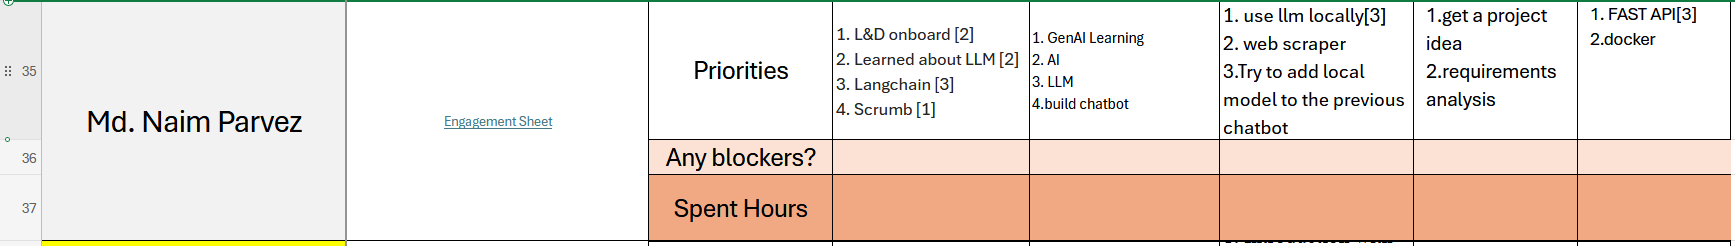
\includegraphics[width=0.95\textwidth]{week1.png}
    \caption{Daily activities log for Week 1}
    \label{fig:week1_log}
\end{figure}

\subsection{Week 2 (March 17 - March 21, 2025)}
\begin{figure}[H]
    \centering
    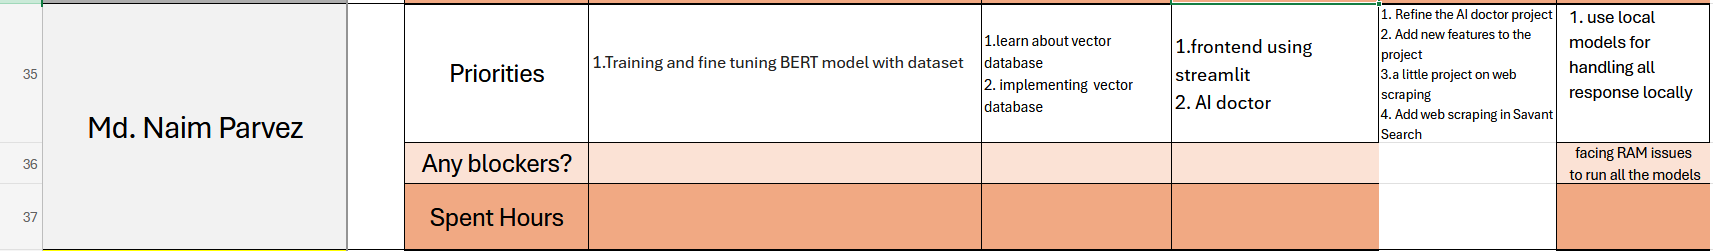
\includegraphics[width=0.95\textwidth]{week2.png}
    \caption{Daily activities log for Week 2}
    \label{fig:week2_log}
\end{figure}

\subsection{Week 3 (March 24 - March 25, 2025)}
\begin{figure}[H]
    \centering
    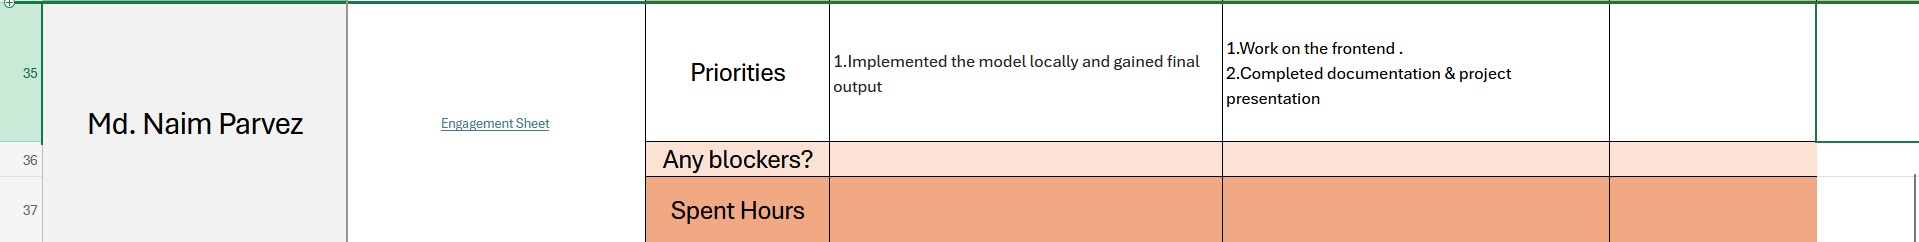
\includegraphics[width=0.95\textwidth]{week3.png}
    \caption{Daily activities log for Week 3}
    \label{fig:week3_log}
\end{figure}
\newpage
\section{Certificate of Completion}

\begin{figure}[H]
    \centering
    
\includegraphics[width=0.95\textwidth, angle=270]{certificate.jpg}
    \caption{Certificate of Completion}
    \label{fig:certificate}
\end{figure}

\end{document}